\chapter{\textbf{Simulaciones de antenas microstrip en forma de serpentina}}\label{ch:simulaciones}

En este capítulo presentaremos la antena de tecnología microstrip con parche radiante en forma de serpentina descrita en el artículo de Soontornpipit~\cite{soont}. En las secciones~\ref{sec:base} y~\ref{sec:original} veremos el análisis y simulación de la antena original del artículo. A continuación, veremos en la sección~\ref{sec:modificado} un diseño modificado de la antena original ajustando algunos parámetros. En último punto, la sección~\ref{sec:optimizado}, analizaremos y simularemos una antena con materiales que se encuentran habitualmente en laboratorios de investigación y con algunos parámetros optimizados a partir del diseño original.


\section{Introducción al diseño base de la antena}\label{sec:base}

Comenzaremos explicando el diseño original del artículo de Soontornpipit. En este artículo el diseño de la antena es muy simple: se trata de una antena microstrip, alimentada por un cable coaxial y que posee una estructura radiante en forma de serpentina, es decir, tiene los brazos plegados entre sí formando varias curvas en ángulo recto. Las dimensiones originales del diseño del parche están recogidas en la \textit{fig. \ref{fig:fig5.1}}. La medida $B$ del último brazo de la estructura de serpentina la toman los autores del artículo como una variable a estudiar a lo largo del mismo. Para nuestro estudio hemos cogido la medida inicial de $B$ que toma el valor de 8.4 mm.

\begin{figure}[!htb]
    \centering
    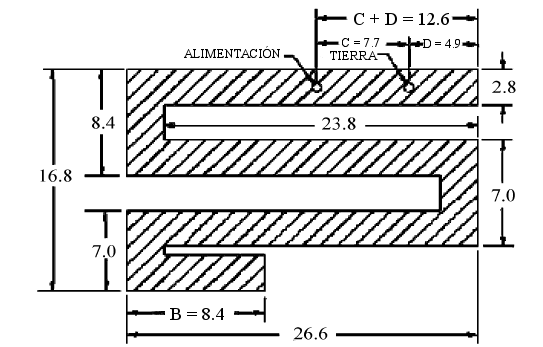
\includegraphics[scale=0.55]{./Simulaciones/original_design2}
    \caption{Medidas originales del diseño de Soontornpipit \cite{serpentina}}
    \label{fig:fig5.1}
\end{figure}

Como podemos ver, las dimensiones de la antena se ajustan a una medida de $\lambda$/4, por lo que la antena queda adaptada sin impedancia imaginaria. Dentro del artículo se hacen distintos estudios como son el cambio de materiales, cambios en el grosor de los substratos e incluso un cambio en el diseño del parche radiante. Todo ello, simulado y comprobado en dos diferentes medios: la antena en entorno de espacio libre y la antena colocada dentro de un bloque rectangular de 2/3 de la permitividad relativa del músculo humano. Los resultados dentro del artículo se ajustan al entorno de trabajo que presentan y cabe destacar que el diseño de la antena es muy simple. Además, los autores del artículo argumentan que su propio artículo es una guía para el diseño de antenas microstrip para DMI.

Al principio del mismo artículo se recoge la posibilidad de utilizar esta antena en un dispositivo desfribilador del corazón o incluso en un marcapasos. Dicha posibilidad es de hecho factible, ya que las dimensiones de la antena son muy reducidas, apenas 3 cm de largo y de ancho. Las medidas de la antena y los materiales utilizados se recogen en las \textit{tablas \ref{tab:tabla5.1}} y~\textit{\ref{tab:tabla5.2}}.

% Tabla medidas originales

\begin{table}[h]
    \centering\scalebox{0.99}{
        \begin{tabular}{| c | c | c | c | c | c |}
            \hline
            \textbf{Dimensiones} & \textbf{mm} & & \textbf{Dimensiones} & \textbf{mm} \\
            \hline
            \hline
            Largo total          & 29.4        & & B                    & 8.4         \\
            \hline
            Alto total           & 19.6        & & C                    & 7.7         \\
            \hline
            Ancho total          & 6.1         & & D                    & 4.9         \\
            \hline
            Largo parche         & 26.6        & & Grosor substratos    & 3           \\
            \hline
            Alto parche          & 16.8        & & Radio pines          & 0.997       \\
            \hline
            Ancho parche         & 2.8         & & Grosor conductor     & 0.1         \\
            \hline
            \hline
        \end{tabular}}
    \caption{Dimensiones originales de la antena de serpentina del artículo de Soontornpipit.}
    \label{tab:tabla5.1}
\end{table}

% Tabla con materiales originales

\begin{table}[h]
    \centering\scalebox{0.99}{
        \begin{tabular}{| c | c | c | c | c | c |}
            \hline
            \textbf{Materiales dieléctricos}   & \textbf{$\epsilon_{r}$} \\
            \hline
            \hline
            Alumina (substrato)                & 9.4                     \\
            \hline
            Macor (superestrato)               & 3.1                     \\
            \hline
            \hline
            \textbf{Parche, masa y conectores} & \textbf{$\sigma$ [S/m]} \\
            \hline
            \hline
            Cobre                              & 5.8 · $10^7$            \\
            \hline
            \hline
        \end{tabular}}
    \caption{Materiales originales de la antena de serpentina del artículo de Soontornpipit.}
    \label{tab:tabla5.2}
\end{table}


\section{Diseño de la antena de serpentina propuesta}\label{sec:original}

Tras estudiar el diseño del artículo, hemos utilizado la herramienta CST Studio Suite para simular el comportamiento de la antena. Vamos a simular la antena en dos ámbitos distintos. El primero será la antena en espacio libre, sin nada alrededor y después simularemos la antena rodeada de músculo, tal y como viene en el artículo.

\subsection{Antena original en espacio libre}\label{subsec:antena-original-en-espacio-libre}

La \textit{fig. \ref{fig:fig5.2}} recoge el diseño en tres dimensiones de la antena sin nada alrededor para facilitar la visualización de su forma.

% ANTENA SERPENTINA ORIGINAL SIN NADA
\begin{figure}[!htb]
    \centering
    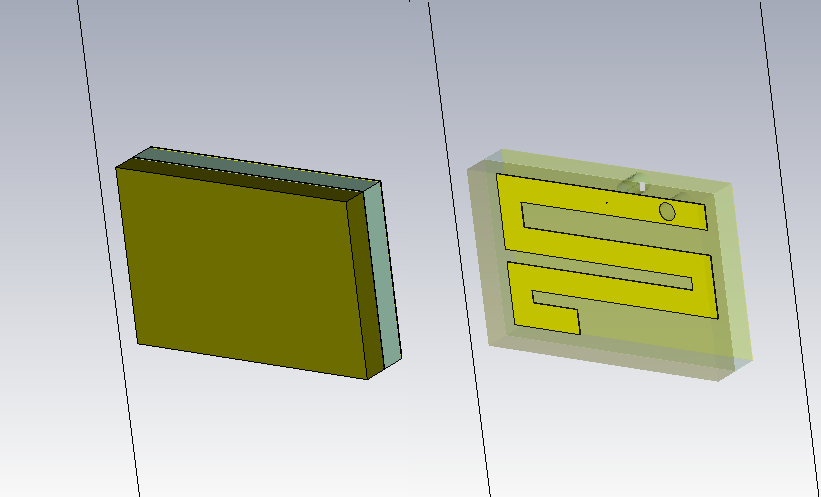
\includegraphics[scale=0.45]{./Simulaciones/original_antenna/original_antenna_copy}
    \caption{Diseño antena original construida en el software CST.}
    \label{fig:fig5.2}
\end{figure}

Al igual que en el artículo, por cada simulación que hagamos, realizaremos un estudio del parámetro $S_{11}$, del diagrama de radiación y de su campo eléctrico radiado. El parámetro $S_{11}$ nos informa sobre las frecuencias a las que la antena radia; el diagrama de radiación nos indicará hacia qué ángulo será más directiva la antena (donde mejor apunta y llega más potencia radiada) y el campo eléctrico nos dirá cómo está radiando la antena.

% S11 ANTENA SERPENTINA ORIGINAL SIN NADA
\begin{figure}[!htb]
    \centering
    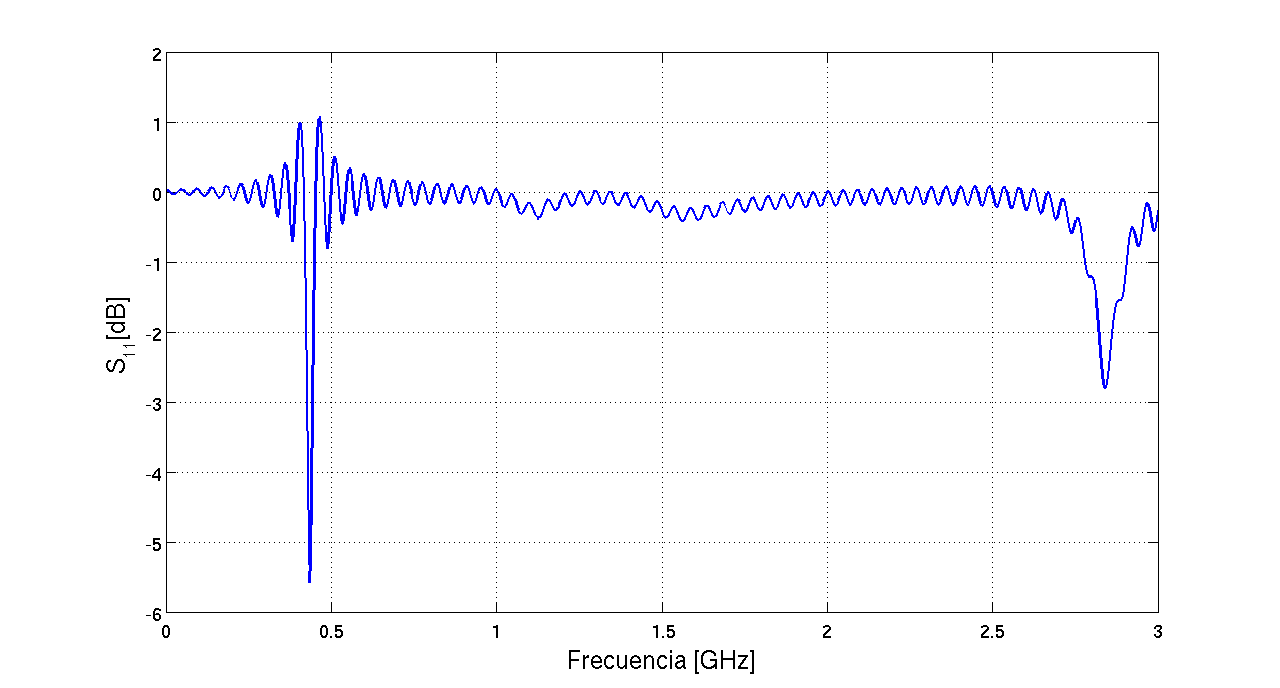
\includegraphics[scale=0.45]{./Simulaciones/matlab2/S11_original_free}
    \caption{Gráfica que recoge el parámetro $S_{11}$ de la antena de serpentina original en espacio libre.}
    \label{fig:fig5.3}
\end{figure}

En primer lugar, presentamos el resultado de la simulación del parámetro $S_{11}$. La \textit{fig. \ref{fig:fig5.3}} muestra que la antena del artículo simulada trabaja en un entorno muy parecido a la banda MICS, aunque en el espacio libre no llega a ser exactamente dicha banda. Las fluctuaciones que vemos en la gráfica se deben a la simulación realizada por el software CST. En comparación con el artículo, tenemos una variación importante, ya que según sus estudios, la banda central para la antena de serpentina en aire es de aproximadamente 370-380 MHz. En nuestro caso, la frecuencia de resonancia es de aproximadamente 435 MHz. Debemos decir que los autores del artículo no citan en ningún momento qué tipo de software han utilizado, por lo que la comparación realmente no llegará a ser exacta; lo único sí mencionado es que utilizan el método FDTD, utilizado también por nuestro software.\\

A continuación vamos a proceder a mostrar el campo eléctrico de la antena original. Para ello, se presentan cuatro figuras: las tres primeras, \textit{fig. \ref{fig:fig5.4}},~\textit{\ref{fig:fig5.5}} y~\textit{\ref{fig:fig5.6}}, son tres modelos en tres dimensiones de la antena y pequeños atributos que marcan la intensidad y dirección del campo; la última, \textit{fig. \ref{fig:fig5.7}} es una representación del campo en el parche radiante.

% E FIELD ANTENA SERPENTINA ORIGINAL SIN NADA
\begin{figure}[!htb]
    \centering
    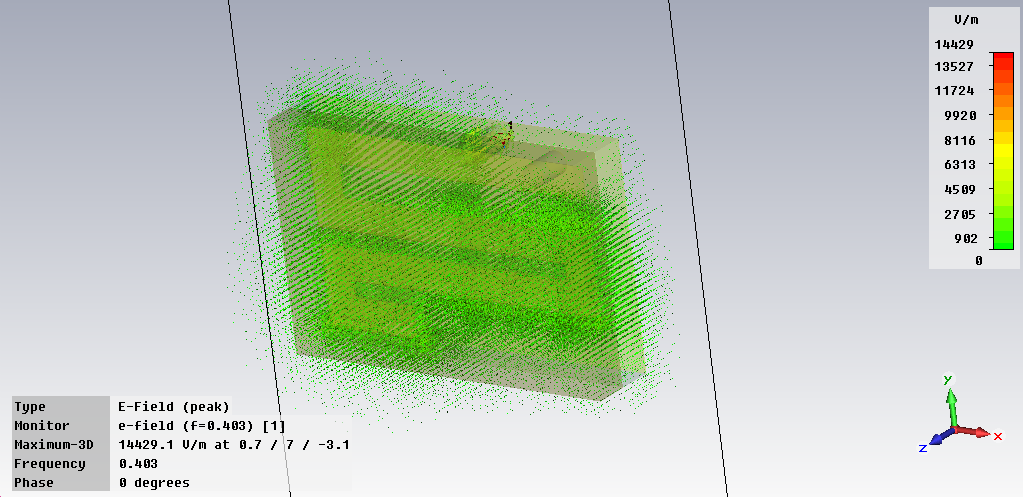
\includegraphics[scale=0.3]{./Simulaciones/original_antenna/original_antenna_E-Field}
    \caption{Representación del campo eléctrico en prespectiva.}
    \label{fig:fig5.4}
\end{figure}

\begin{figure}[!htb]
    \centering
    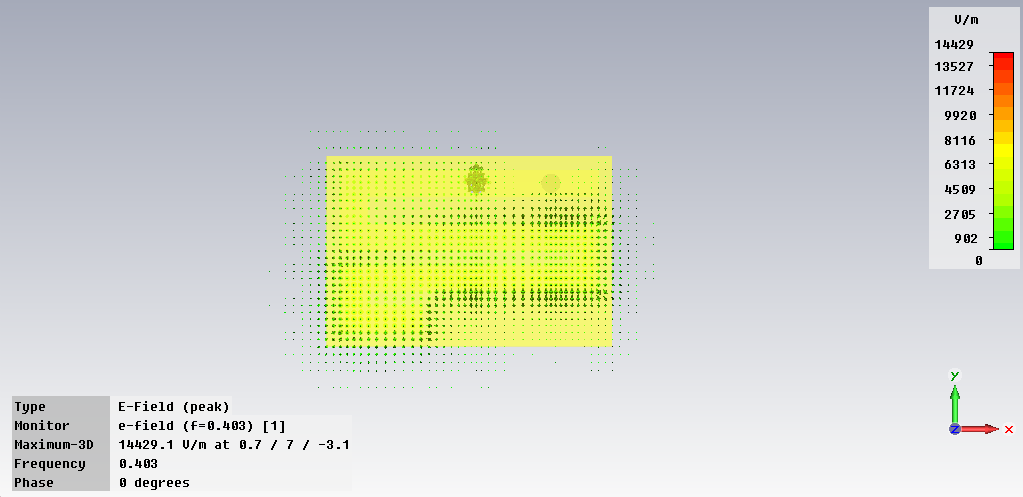
\includegraphics[scale=0.3]{./Simulaciones/original_antenna/original_antenna_E-Field_2}
    \caption{Representación del campo eléctrico desde el frente.}
    \label{fig:fig5.5}
\end{figure}

\begin{figure}[!htb]
    \centering
    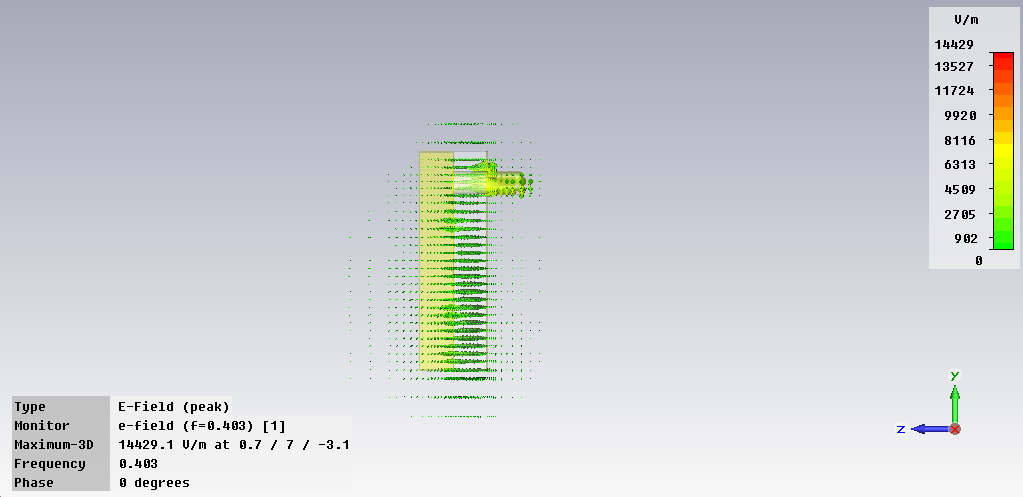
\includegraphics[scale=0.3]{./Simulaciones/original_antenna/original_antenna_E-Field_3}
    \caption{Representación del campo eléctrico desde el lado derecho.}
    \label{fig:fig5.6}
\end{figure}

\begin{figure}[!htb]
    \centering
    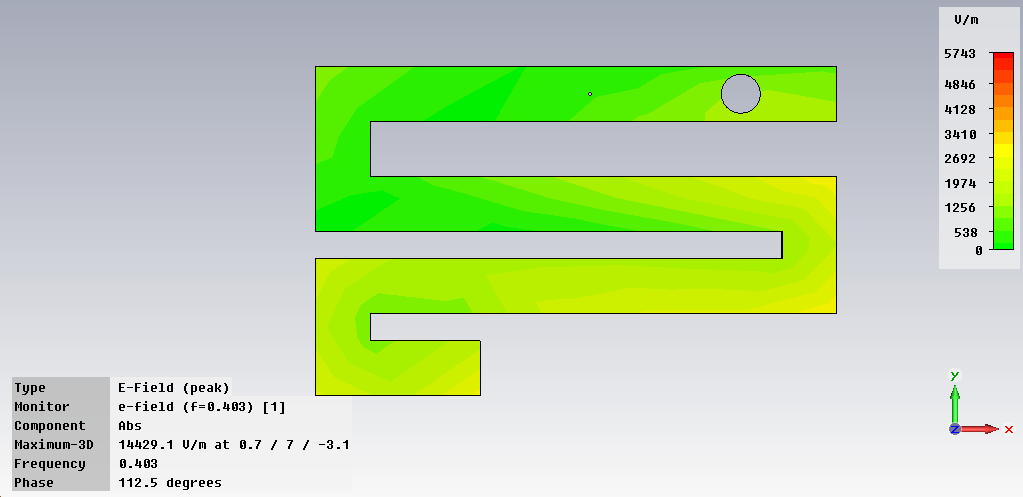
\includegraphics[scale=0.3]{./Simulaciones/original_antenna/original_antenna_E-Field_4}
    \caption{Representación del campo eléctrico justo en el parche radiante.}
    \label{fig:fig5.7}
\end{figure}

\clearpage

Como podemos ver, la antena radia campo eléctrico al exterior y sobre todo, si nos fijamos en las \textit{figs. \ref{fig:fig5.5}} y~\textit{\ref{fig:fig5.7}}, en la parte final de la serpentina. La representación del campo eléctrico en el artículo es muy parecida aunque no tenemos tanto detalles como en las imágenes anteriores.\\

Lo último que nos queda por ver es el diagrama de radiación. Tras la simulación encontramos que la antena es capaz de radiar con dos lóbulos principales tal y como podemos apreciar en la siguiente figura.

% DIAGRAMA DE RADIACION ANTENA SERPENTINA ORIGINAL SIN NADA
\begin{figure}[!htb]
    \centering
    \subfigure[]{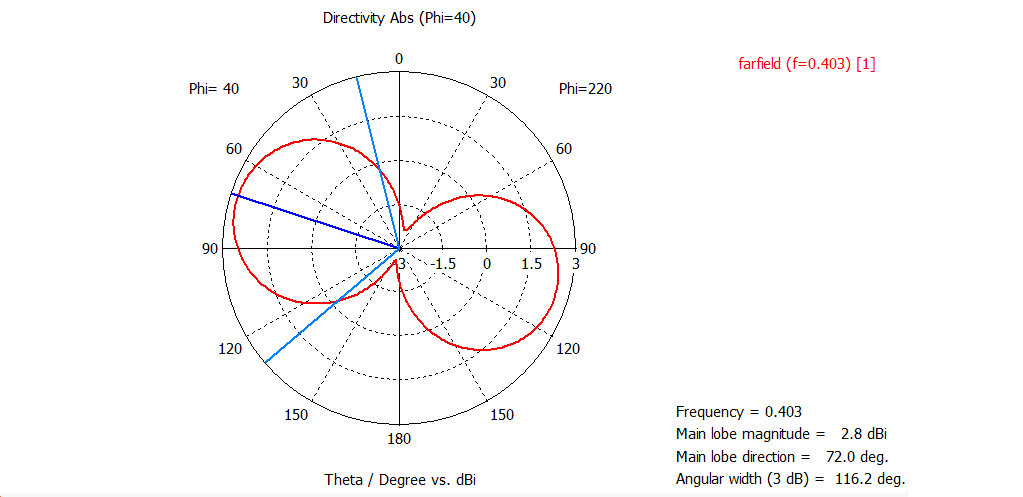
\includegraphics[scale=0.35]{./Simulaciones/original_antenna/original_antenna_radiation_pattern}}
    \subfigure[]{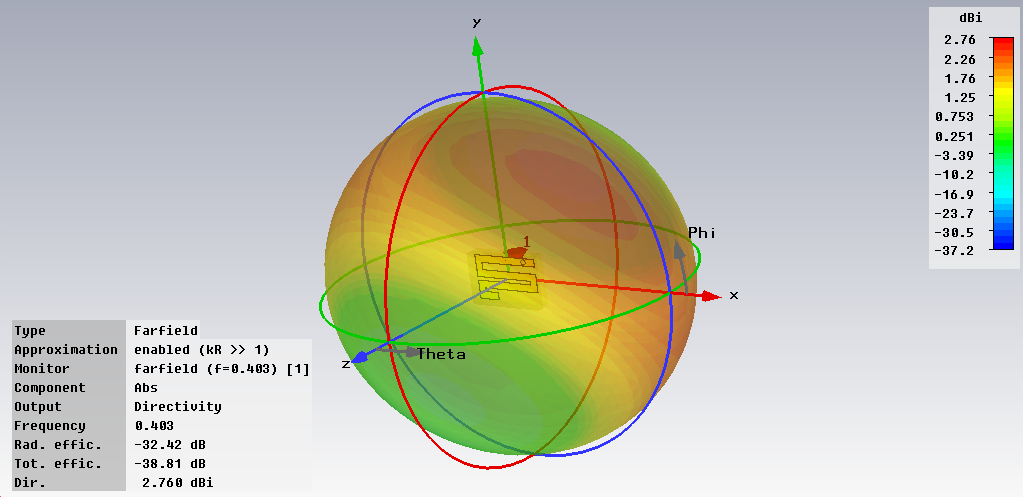
\includegraphics[scale=0.35]{./Simulaciones/original_antenna/original_antenna_radiation_pattern_3D}}
    \caption{Representación del diagrama de radiación de la antena original en espacio libre. En (a) coordenadas polares en 2D manteniendo $\phi$ = 40º y en (b) en 3D.}
    \label{fig:fig5.8}
\end{figure}

\clearpage

\subsection{Antena original rodeada de un bloque de músculo}\label{subsec:antena-original-rodeada-de-un-bloque-de-musculo}

Después de ver los distintos resultados de la antena original en espacio libre, procedemos a simular dicha antena dentro de un bloque de músculo. El diseño del artículo está pensado para esta opción, es decir, situar la antena dentro del cuerpo humano. En esta ocasión, hemos diseñado un bloque rectangular de músculo con el software CST en el cual hemos insertado la antena. Las propiedades dieléctricas del espacio cambian considerablemente, como podremos ver en las simulaciones.

Las propiedades del músculo construido son las siguientes:

% Tabla medidas músculo

\begin{table}[h]
    \centering\scalebox{0.99}{
        \begin{tabular}{| c | c | c | c | c | c |}
            \hline
            \textbf{Dimensiones}             & \textbf{mm} \\
            \hline
            \hline
            Largo                            & 50          \\
            \hline
            Alto                             & 40          \\
            \hline
            Ancho                            & 20          \\
            \hline
            \hline
            \textbf{Permitividad}            &             \\
            \textbf{relativa $\epsilon_{r}$} & 42.807      \\
            \hline
            \hline
            \textbf{Conductividad}           &             \\
            \textbf{eléctrica $\sigma$}      & 0.6463 S/m  \\
            \hline
            \hline
        \end{tabular}}
    \caption{Propiedades del bloque de músculo diseñado para su simulación.}
    \label{tab:tabla5.3}
\end{table}

En primer lugar, en la \textit{fig. \ref{fig:fig5.9}}, presentamos el diseño de la antena dentro del bloque de músculo. Como se aprecia en la imagen, lo único que cambia es el bloque rectangular que rodea la antena.

% ANTENA ORIGINAL EN MUSCULO
\begin{figure}[!htb]
    \centering
    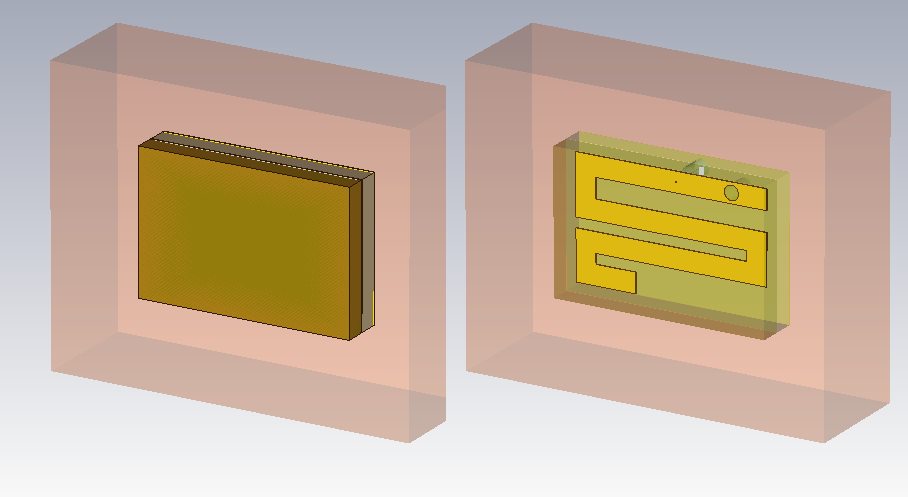
\includegraphics[scale=0.25]{./Simulaciones/original_antenna_muscle/original_serpentine_muscle_copy}
    \caption{Diseño antena original insertada en un bloque de músculo construida en el software CST.}
    \label{fig:fig5.9}
\end{figure}

\clearpage

La simulación del parámetro $S_{11}$ se recoge en la \textit{fig. \ref{fig:fig5.10}}.

% S11 ANTENA ORIGINAL EN MUSCULO
\begin{figure}[!htb]
    \centering
    \subfigure[]{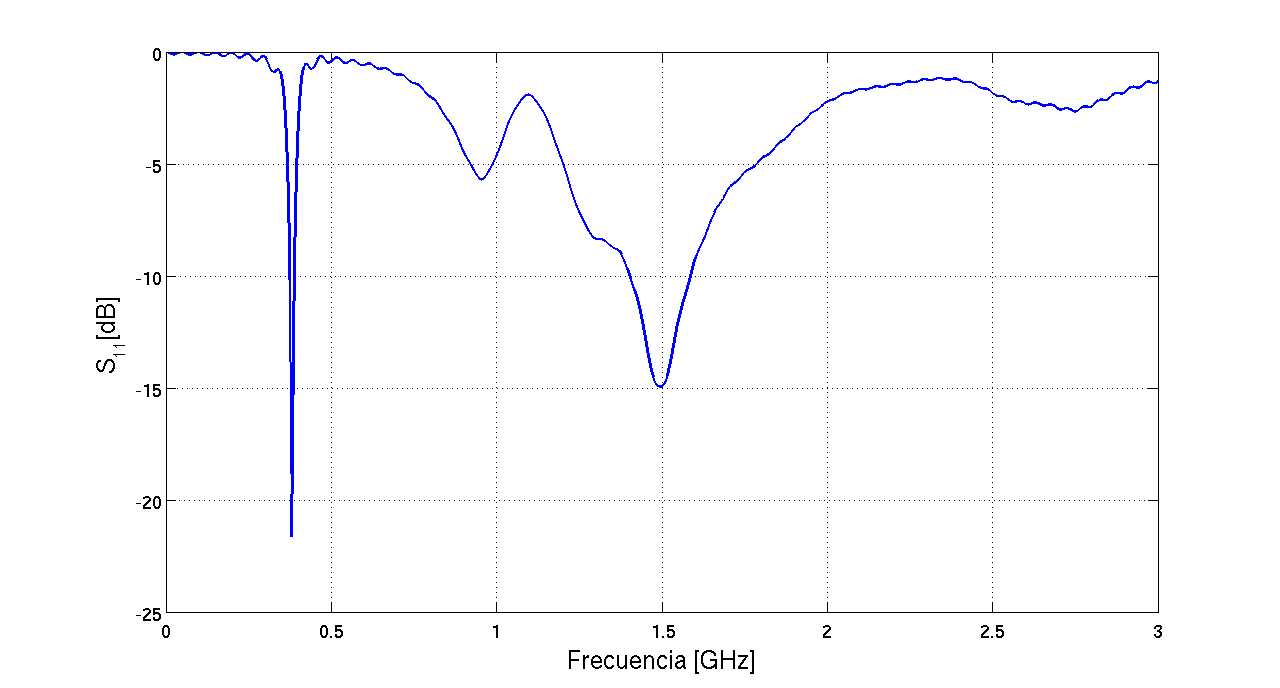
\includegraphics[scale=0.4]{./Simulaciones/matlab2/S11_original_muscle}}
    \subfigure[]{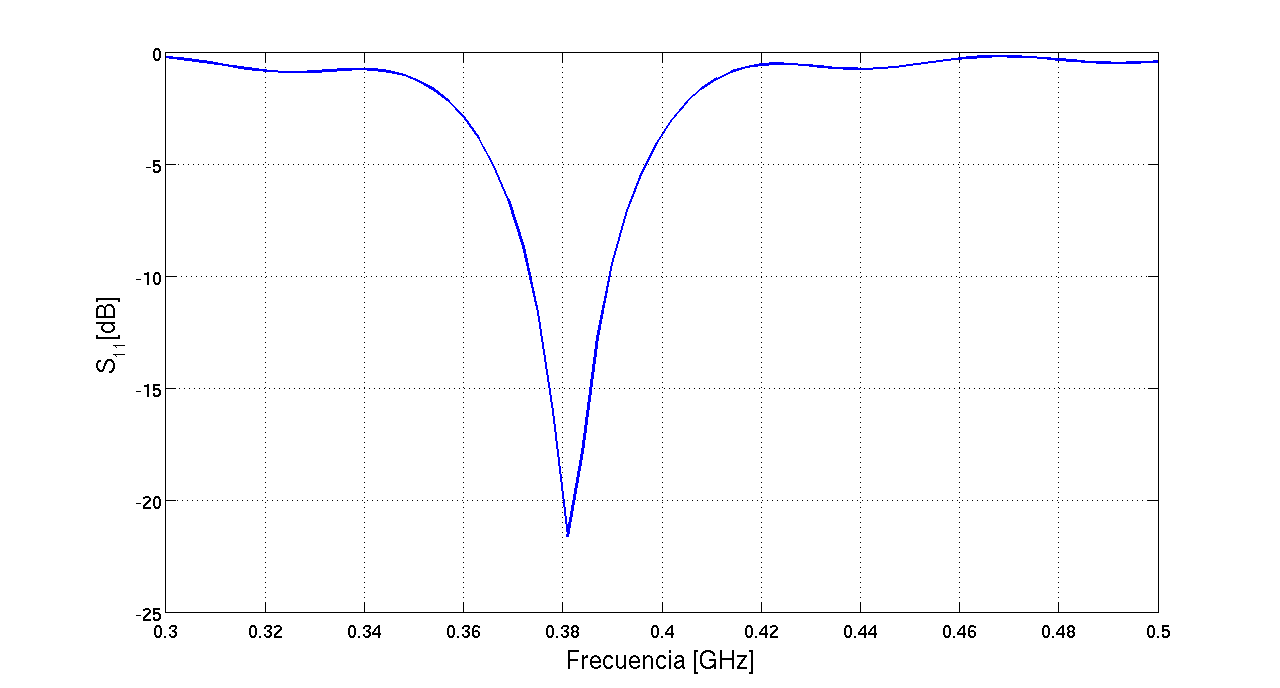
\includegraphics[scale=0.4]{./Simulaciones//matlab2/S11_original_muscle_zoom}}
    \caption{Gráficas que recogen el parámetro $S_{11}$ de la antena de serpentina original rodeada de músculo. En (a) medidas simuladas de 0 a 3 GHz y en (b) se ha aplicado un zoom en la banda MICS.}
    \label{fig:fig5.10}
\end{figure}

Las gráficas de la \textit{fig. \ref{fig:fig5.10}} dejan patente que la antena diseñada en el artículo permite trabajar en una banda cercana a la banda MICS, pero no exactamente en la misma banda. En el artículo, los autores proporcionan datos que sitúan esta antena simulada, en un entorno muy parecido o prácticamente igual en el que estamos trabajando, en una banda cercana a los 500 MHz, muy lejos de nuestra banda de trabajo. Sin embargo, nuestra simulación se acerca mucho más a la banda y como podemos apreciar en la gráfica zoom, \textit{fig. \ref{fig:fig5.10} (b)}, el mínimo $S_{11}$ está a escasos 20 MHz de la banda MICS, donde tenemos -3.02 dB de dicho parámetro. Por lo tanto, unas de las razones que nos empuja a seguir estudiando y considerando este diseño es centrar el mínimo valor de $S_{11}$ a la banda MICS. Como se anunció anteriormente, estas desigualdades entre el artículo y nuestra simulación son seguramente debidas a que no se usan el mismo software o quizá no estamos considerando algún parámetro extra que los autores no señalan.

Procedemos a ver el campo eléctrico de esta simulación, junto a la pérdida de potencia en el superestrato diélectrico de la antena y el diagrama de radiación.

%CAMPO ELÉCTRICO Y PÉRDIDA DE POTENCIA
\begin{figure}[!htb]
    \centering
    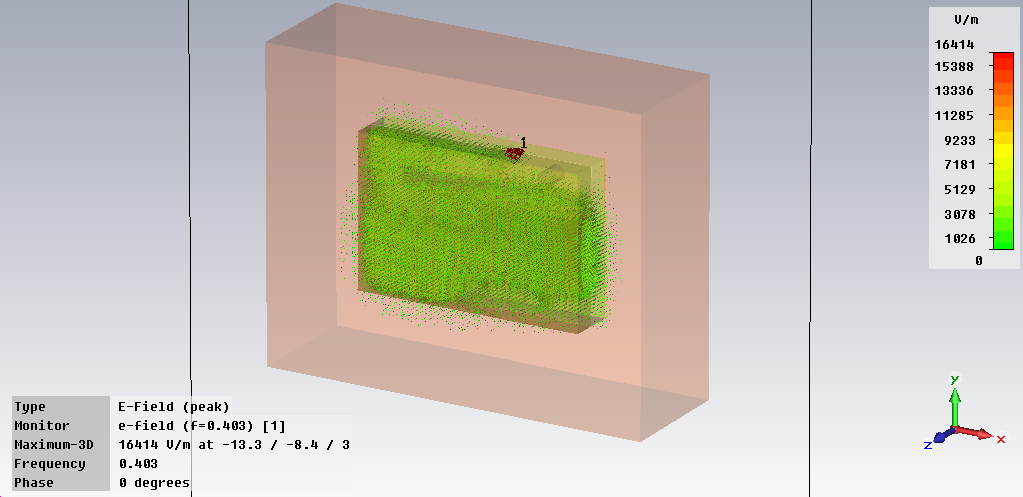
\includegraphics[scale=0.3]{./Simulaciones/original_antenna_muscle/original_serpentine_muscle_E-Field}
    \caption{Representación campo eléctrico en prespectiva.}
    \label{fig:fig5.11}
\end{figure}

\begin{figure}[!htb]
    \centering
    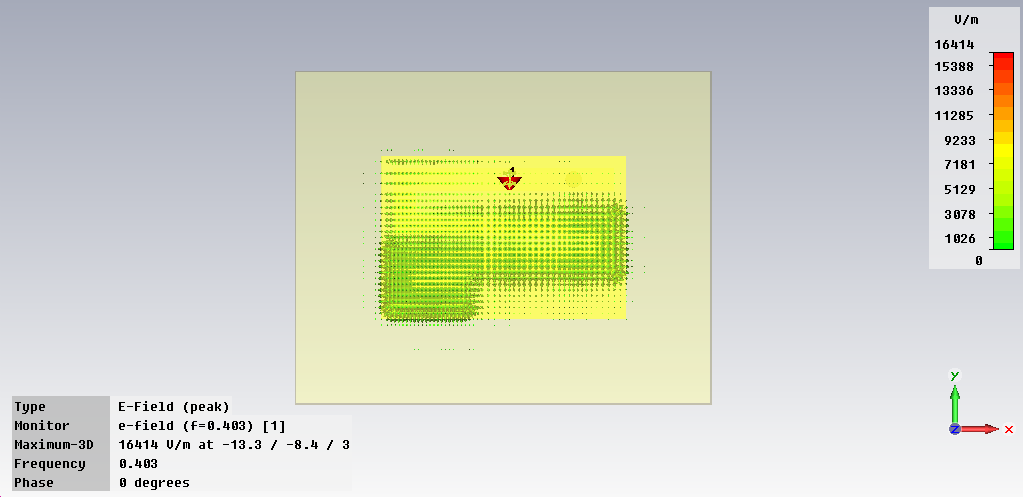
\includegraphics[scale=0.3]{./Simulaciones/original_antenna_muscle/original_serpentine_muscle_E-Field_2}
    \caption{Representación campo eléctrico desde el frente.}
    \label{fig:fig5.12}
\end{figure}

\begin{figure}[!htb]
    \centering
    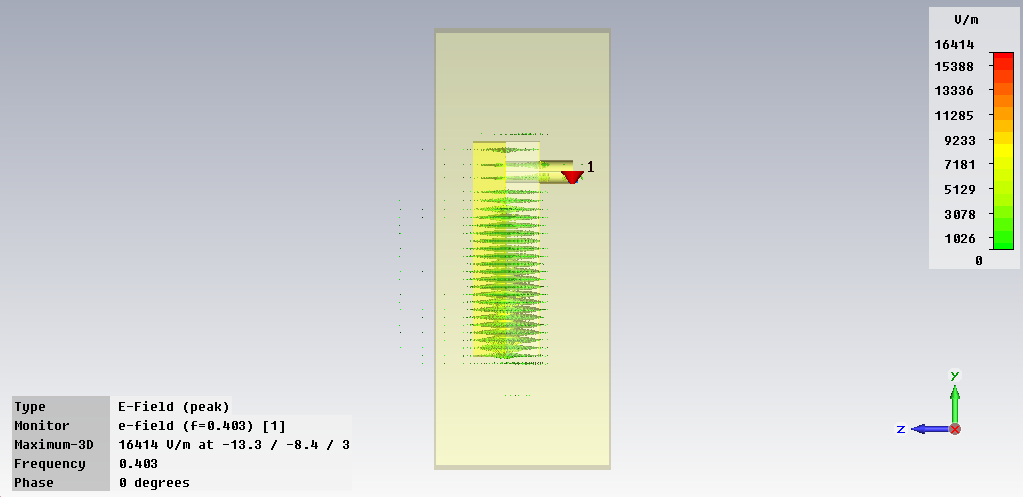
\includegraphics[scale=0.3]{./Simulaciones/original_antenna_muscle/original_serpentine_muscle_E-Field_3}
    \caption{Representación campo eléctrico desde el lado derecho.}
    \label{fig:fig5.13}
\end{figure}

\begin{figure}[!htb]
    \centering
    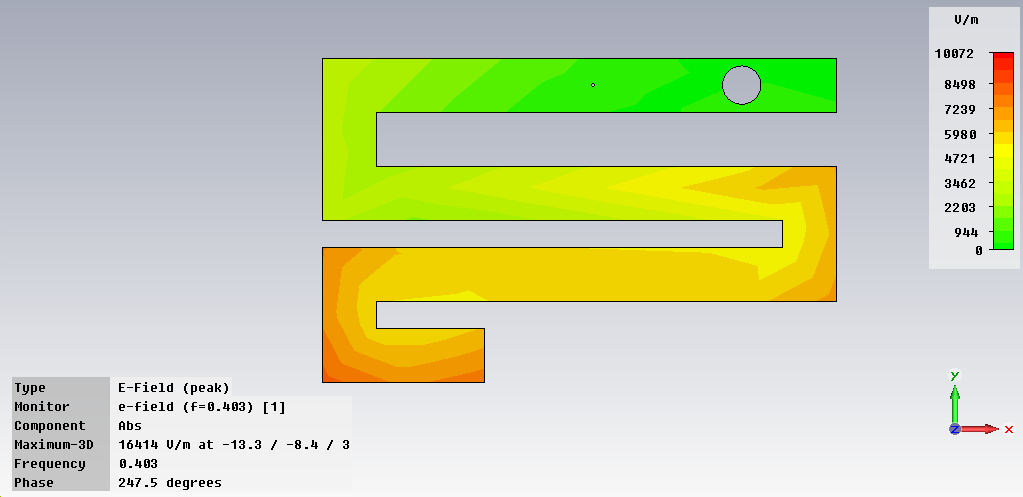
\includegraphics[scale=0.3]{./Simulaciones/original_antenna_muscle/original_serpentine_muscle_E-Field_4}
    \caption{Representación campo eléctrico justo en el parche radiante.}
    \label{fig:fig5.14}
\end{figure}

\begin{figure}[!htb]
    \centering
    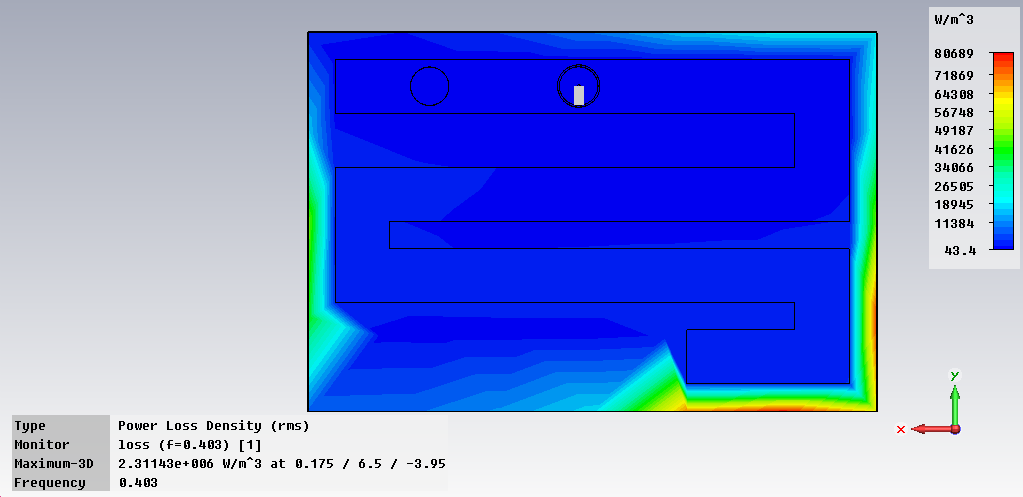
\includegraphics[scale=0.4]{./Simulaciones/original_antenna_muscle/original_serpentine_muscle_power_loss}
    \caption{Representación pérdida de potencia en el superestrato diélectrico.}
    \label{fig:fig5.15}
\end{figure}

\newpage

Las imágenes mostradas en las \textit{figs. \ref{fig:fig5.11}},~\textit{\ref{fig:fig5.12}},~\textit{\ref{fig:fig5.13}} y~\textit{\ref{fig:fig5.14}}, reflejan cómo el campo eléctrico se distribuye alrededor de la antena, enfatizando la densidad del mismo en la región inferior. En la \textit{fig. \ref{fig:fig5.14}} se puede ver cómo ha aumentado el campo eléctrico radiado a través del parche en comparación a exponer la antena al espacio libre, \textit{fig. \ref{fig:fig5.7}}. La misma comparación es observada en las distintas figuras representadas en tres dimensiones, demostrando que la antena es más efectiva en un medio dieléctrico como el músculo que en el espacio libre.

La imagen representada en \textit{fig. \ref{fig:fig5.15}} muestra la pérdida de potencia en el superstrato dieléctrico. Nos indica concretamente en qué zonas radia la antena al exterior y por dónde se está perdiendo eficiencia en cuanto a la potencia total entregada a la propia antena.

El diagrama de radiación de la antena rodeada de músculo queda de la siguiente manera:

\begin{figure}[!htb]
    \centering
    \subfigure[]{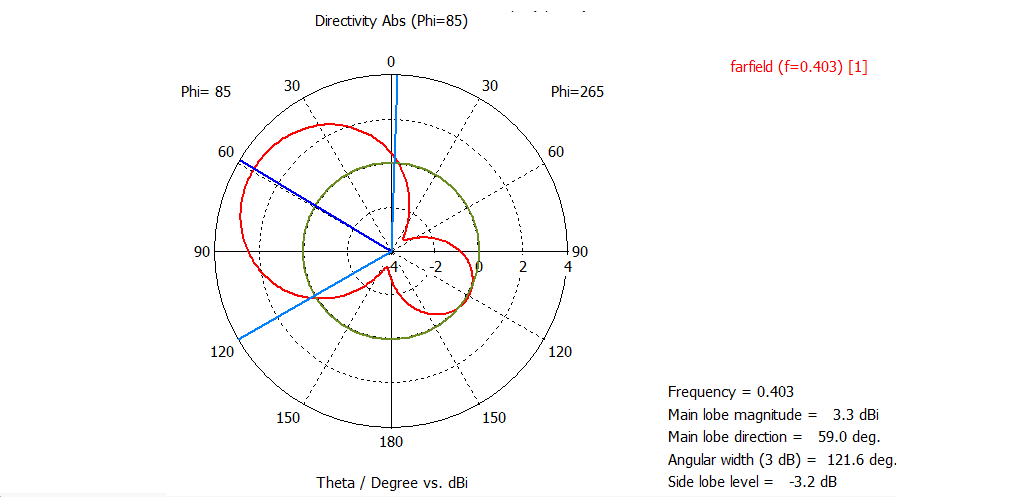
\includegraphics[scale=0.3]{./Simulaciones/original_antenna_muscle/original_serpentine_muscle_radiation_pattern}}
    \subfigure[]{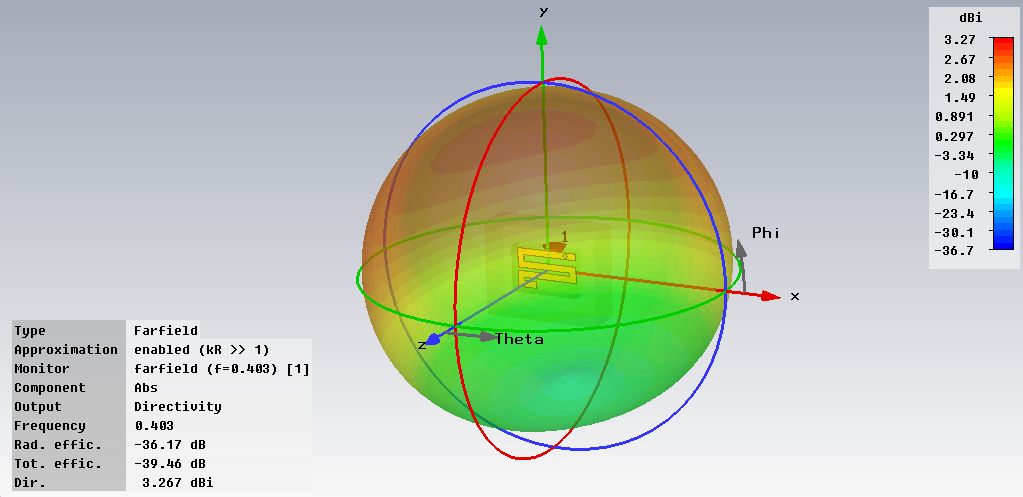
\includegraphics[scale=0.3]{./Simulaciones/original_antenna_muscle/original_serpentine_muscle_radiation_pattern_3D}}
    \caption{Representación del diagrama de radiación de la antena original en tejido muscular. En (a) coordenadas polares en 2D manteniendo $\phi$ = 85º y en (b) en 3D.}
    \label{fig:fig5.16}
\end{figure}

Ha habido un cambio notable frente al diagrama de radiación de la antena en espacio libre: ya no existen dos lóbulos principales bien diferenciados. En su lugar, el lóbulo principal se ha situado en 60º $\theta$ aproximadamente, dejando fijo $\phi$ a 85º, y el lóbulo posterior se ha visto reducido. Además la antena radia hacia el frente con valor de ganancia 3.3 dBi, alto con respecto a la eficiencia pérdida por potencia.
En esta última figura se ve claramente la zona roja, de máxima radiación, situada en una zona superior a la antena, como bien dice el diagrama de radiación en coordenadas polares, a 60º aproximadamente de la normal de la antena.\\

Hemos comprobado mediante simulación realizada por sofrware de computadora cómo funciona la antena del artículo de Soontorpipit. Según nuestras simulaciones, esta antena puede ser expuesta a muchas modificaciones para su correcto funcionamiento en la banda MICS e incluso mejorar su eficiencia en dicha banda. A continuación, vamos a tomar esta antena como referencia y modificar ciertos parámetros que incluso los autores proponen como mejora en sus conclusiones.


\section{Estudio paramétrico de la antena de serpentina propuesta}\label{sec:modificado}

La idea que hemos dejado plasmada en el anterior párrafo la debemos llevar a cabo modificando en primer lugar las dimensiones del parche radiante, la estructura de serpentina en sí. Como sabemos del artículo, existen tres medidas catalogadas por los autores como B, C y D. Dichas medidas corresponden con la longitud del último brazo, la distancia entre el pin de tierra y el pin de alimentación y la distancia entre el principio de la estructura y el pin de tierra respectivamente. Originalmente, las medidas son: \textbf{B = 8.4 mm, C = 7.7 mm y D = 4.9 mm}.

Los estudios que se han realizado en simulación de una posible antena modificada quedan reflejados en la siguiente tabla, donde se expone qué se ha cambiado y qué resultados se han obtenido. Los materiales son los mismos con los que se ha simulado la antena original, únicamente se ha modificado las dimensiones del parche radiante. Huelga decir que se ha intentado desde el primer momento tanto mejorar el parámetro $S_{11}$ como centrar la frecuencia de resonancia a la banda MICS; además, todas las simulaciones para encontrar el diseño definitivo se han hecho con la antena rodeada de un bloque de músculo.

% TABLA DIFERENTES RESULTADOS

\begin{table}[h]
    \centering\scalebox{0.85}{
        \begin{tabular}{| c | c | c | c | c | c |}
            \hline
            %\fcolorbox{orange}{orange}{ \color{white} LaTeX}
            \textbf{Parámetro modificado} & \textbf{Frecuencia de resonancia} & \textbf{Parámetro $S_{11}$} & \textbf{Ganancia} \\
            \hline
            \hline
            B = 5 mm                      & 393 MHz                           & -26.27 dB                   & 2.8 dBi                           \\
            \hline
            B = 4.5 mm                    & 393 MHz                           & -32.65 dB                   & 2.6 dBi                           \\
            \hline
            B = 4.5 mm                    &                                   &                             &                                   \\
            D = 6 mm                      & 402 MHz                           & -25.27 dB                   & 2.6 dBi                           \\
            \hline
            B = 4.5 mm                    &                                   &                             &                                   \\
            D = 7 mm                      & 408 MHz                           & -25.78 dB                   & 2.6 dBi                           \\
            \hline
            B = 4.5 mm                    &                                   &                             &                                   \\
            D = 6.5 mm                    & 402 MHz                           & -25.43 dB                   & 2.6 dBi                           \\
            \hline
            B = 4.5 mm                    &                                   &                             &                                   \\
            C = 7.8 mm                    & 402 MHz                           & -25.87 dB                   & 2.6 dBi                           \\
            D = 6.5 mm                    &                                   &                             &                                   \\
            \hline
            \textbf{B = 6 mm}             &                                   &                             &                                   \\
            \textbf{C = 7.8 mm}           & \textbf{402 MHz}                  & \textbf{-41.7 dB}           & \textbf{2.7 dBi ($\theta$ = 85º)} \\
            \textbf{D = 7 mm}             &                                   &                             &                                   \\
            \hline
            \hline
        \end{tabular}}
    \caption{Pruebas realizadas para modificar el diseño original de la antena de serpentina.}
    \label{tab:tabla5.4}
\end{table}

En esta tabla, podemos ver las distintas modificaciones que se han realizado al parche de serpentina hasta conseguir unos valores óptimos con un parámetro $S_{11}$ de -41.7 dB a 402 MHz. Los parámetros de ancho y largo de los substratos tampoco se han visto modificados. Vamos a proceder a simular la antena con las últimas características, \textbf{B = 6 mm, C = 7.8 mm, D = 7 mm}, tanto en espacio libre como en músculo. Añadiremos un tercer punto de estudio con una estructura de tres capas, piel, grasa y músculo, intentando simular lo máximo posible un entorno real.

\subsection{Antena modificada en espacio libre}\label{subsec:antena-modificada-en-espacio-libre}

En nuestro software CST para modificar la antena origianl únicamente tenemos que cambiar los parámetros globales que tenemos definidos como B, C y D. Tras cambiar las variables, el diseño se actualiza automáticamente, presentando un nuevo aspecto como se ve en la \textit{fig. \ref{fig:fig5.17}}. Quizá no se aprecia bien los cambios, pero hemos de recordar que modificamos milímetros, apenas apreciables a simple vista; no obstante si se compara con el diseño anterior se ve que el último brazo se ha reducido y la distancia entre pines también ha cambiado.

% ANTENA MODIFICADA
\begin{figure}[!htb]
    \centering
    \subfigure[]{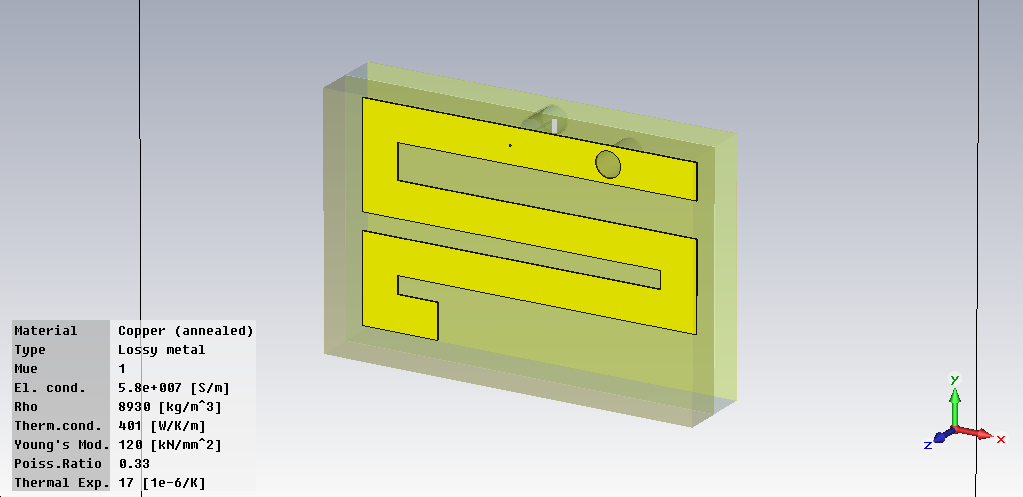
\includegraphics[scale=0.35]{./Simulaciones/tunned_antenna/tunned_serpentine_antenna}}
    \subfigure[]{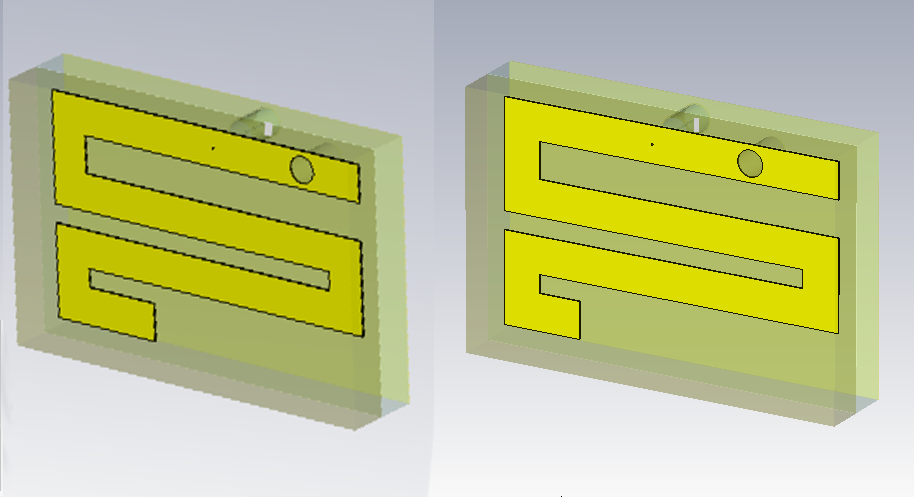
\includegraphics[scale=0.35]{./Simulaciones/tunned_antenna/antenna_comparacion}}
    \caption{Antena microstrip en forma de serpentina modificada. En (a) el diseño completo y en (b) comparación entre la antena original (izquierda) y la modificada (derecha).}
    \label{fig:fig5.17}
\end{figure}

El parámetro $S_{11}$ en este caso, simulación en espacio libre, tiene una forma similar al que presentamos en la sección anterior, con sus impulsos debidos al software y su frecuencia desviada. Incluso en esta ocasión, su frecuencia de resonancia es más alta, como se ven en la \textit{fig. \ref{fig:fig5.19}}, debido seguramente a que hemos acortado la longitud del parche radiante, que es el que fundamentalmente marca dicha frecuencia. En definitiva, pasamos de tener una frecuencia de resonancia de 435 MHz a 456 MHz.

% S11 ANTENA MODIFICADA
\begin{figure}[!htb]
    \centering
    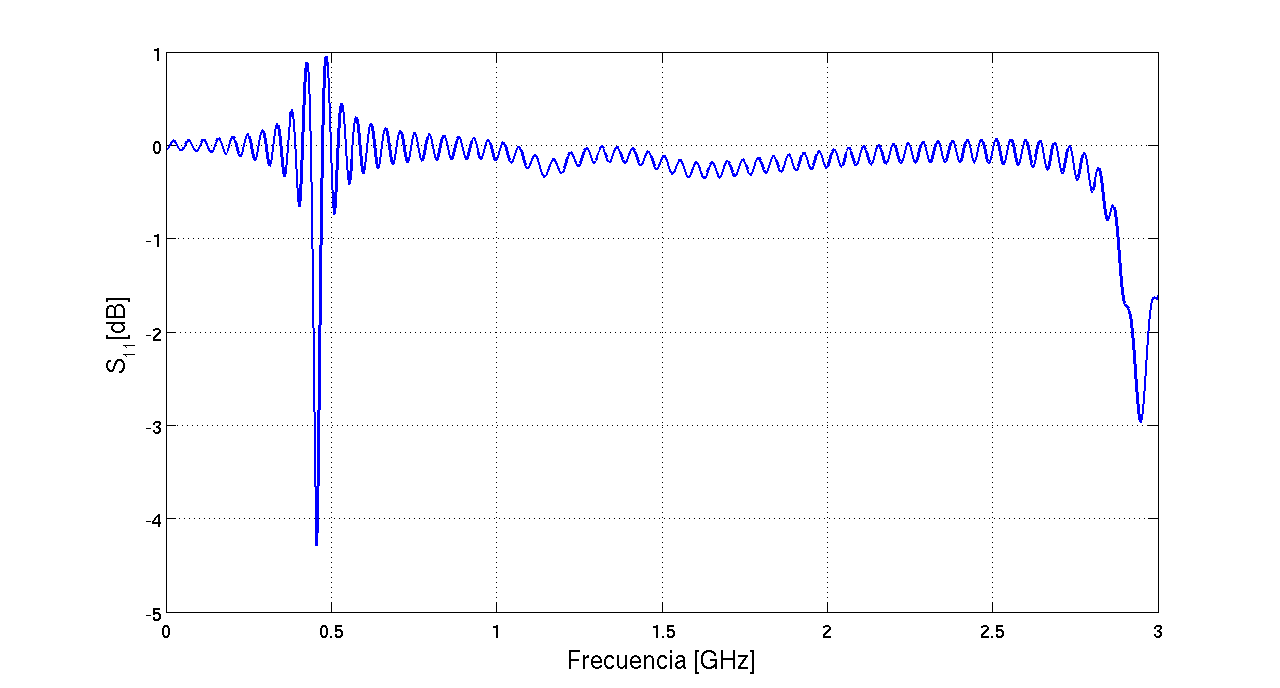
\includegraphics[scale=0.45]{./Simulaciones/matlab2/S11_tunned_free}
    \caption{Gráfica que recoge el parámetro $S_{11}$ de la antena de serpentina modificada en espacio libre.}
    \label{fig:fig5.18}
\end{figure}

\begin{figure}[!htb]
    \centering
    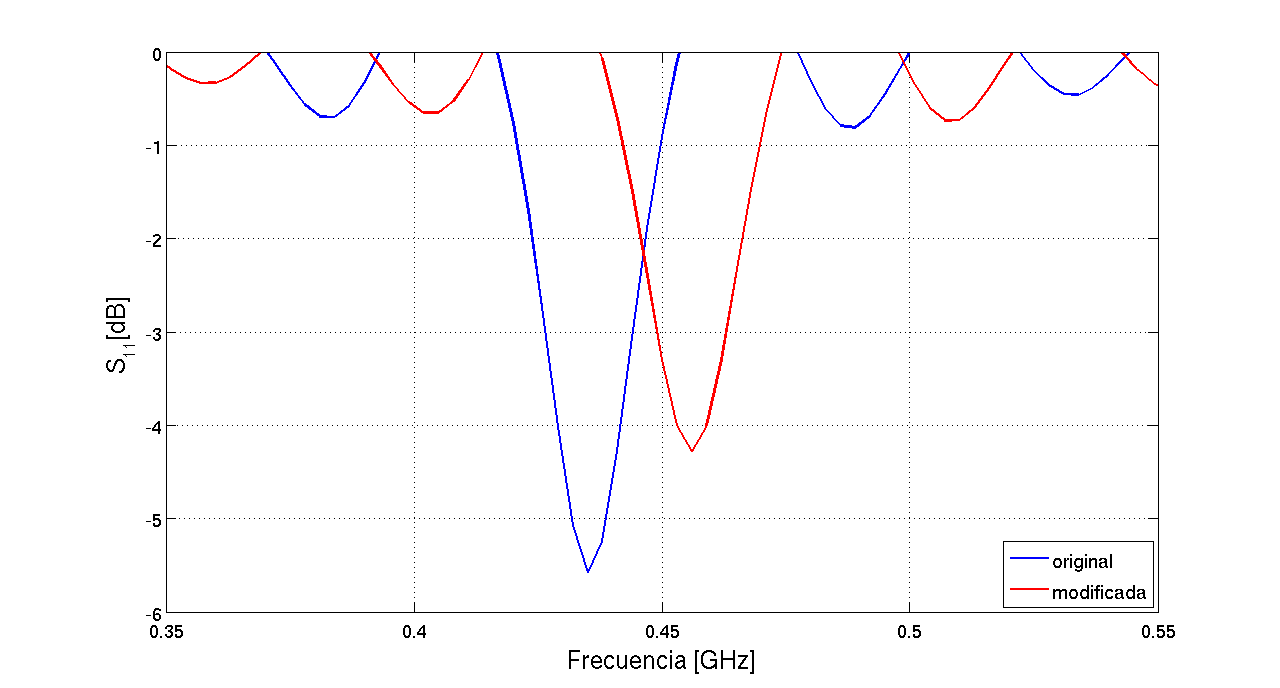
\includegraphics[scale=0.45]{./Simulaciones/matlab2/S11_vs_original_tunned_free_zoom}
    \caption{Gráfica zoom que recoge el parámetro $S_{11}$ de las antenas original y modificada en espacio libre.}
    \label{fig:fig5.19}
\end{figure}

\clearpage

El campo eléctrico para nuestra antena modificada en espacio libre queda muy similar a la antena original. En la \textit{fig. \ref{fig:fig5.20}} se exponen cuatro imágenes del resultado.

% E FIELD ANTENA MODIFICADA
\begin{figure}[!htb]
    \centering
    \subfigure[]{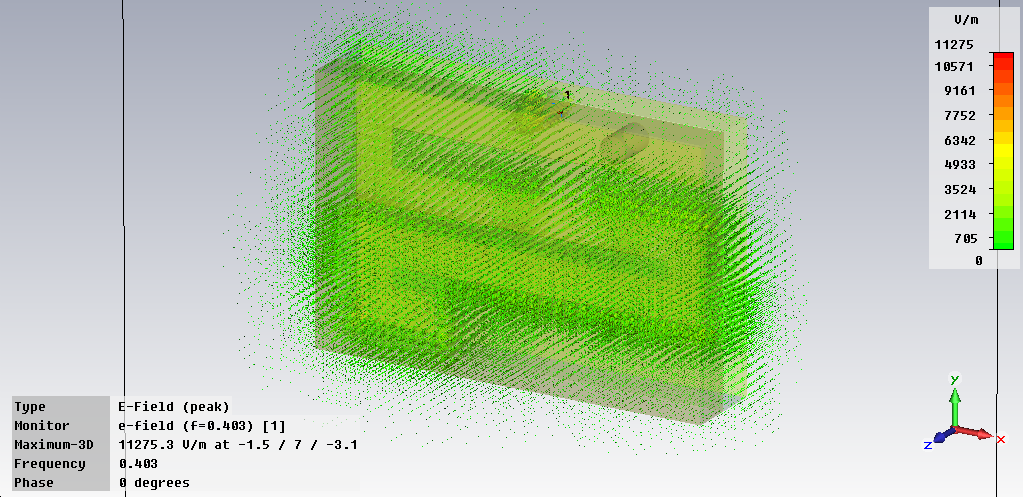
\includegraphics[scale=0.25]{./Simulaciones/tunned_antenna/tunned_serpentine_antenna_E-Field}}
    \subfigure[]{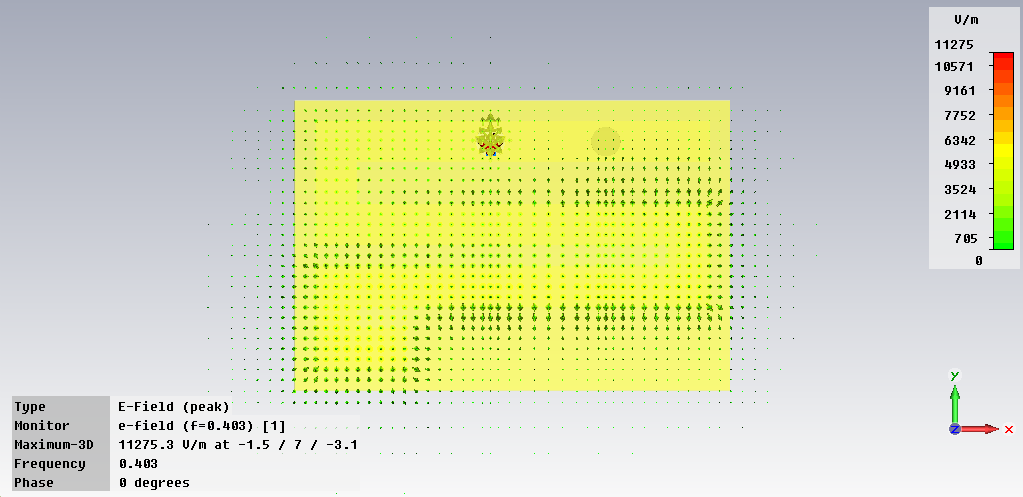
\includegraphics[scale=0.25]{./Simulaciones/tunned_antenna/tunned_serpentine_antenna_E-Field_2}}
    \subfigure[]{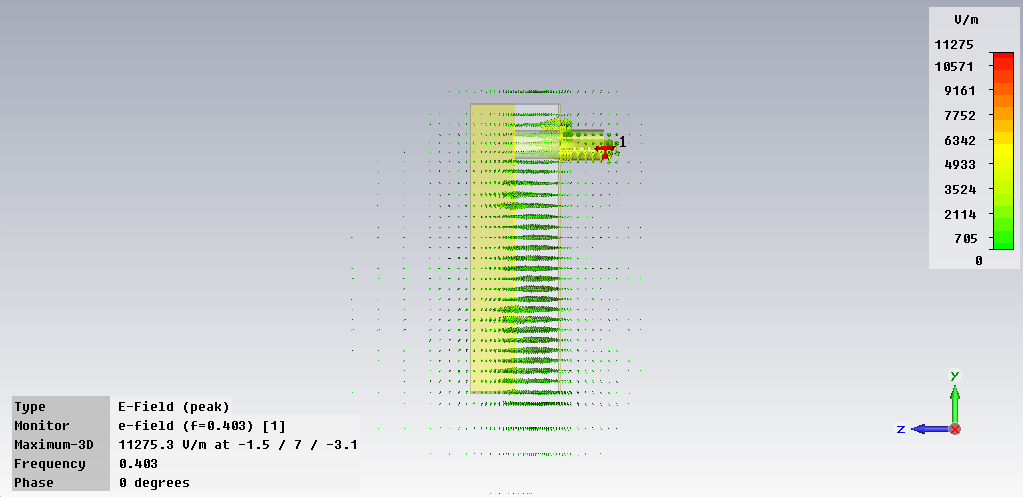
\includegraphics[scale=0.25]{./Simulaciones/tunned_antenna/tunned_serpentine_antenna_E-Field_3}}
    \subfigure[]{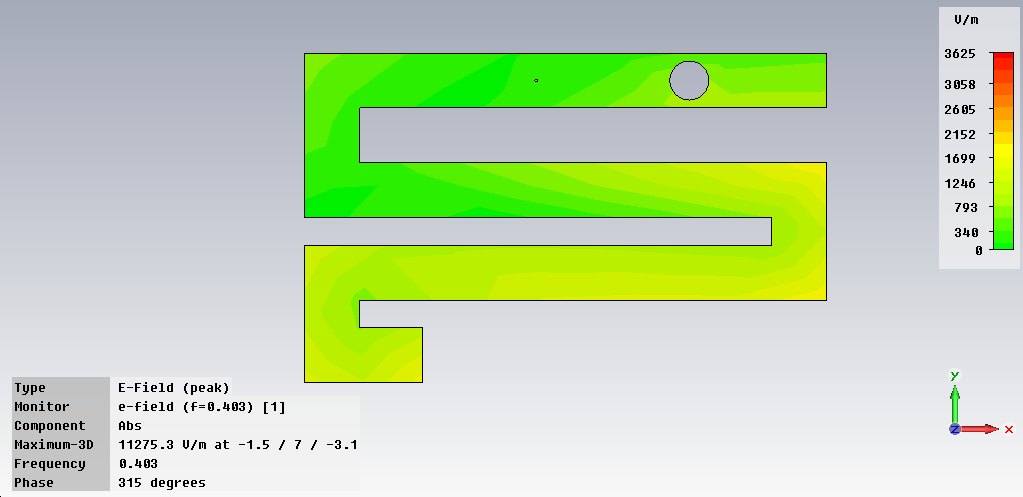
\includegraphics[scale=0.25]{./Simulaciones/tunned_antenna/tunned_serpentine_antenna_E-Field_4}}
    \caption{Representación del campo eléctrico de la antena modificada en espacio libre. En (a) vista en prespectiva; en (b) vista frontal; en (c) vista desde el lado derecho y en (d) vista del parche radiante.}
    \label{fig:fig5.20}
\end{figure}

Como venimos haciendo hasta ahora, representamos además el diagrama de radiación correspondiente. Éste ha cambiado respecto al original del artículo, ya que los lóbulos han modificado su posición y se encuentran en otra ángulo $\theta$ respecto a $\phi$, fijado en aproximadamente 215º. Sin embargo, el propio software de CST nos indica que este diseño no es adecuado, ya que la radiación efectiva es muy baja, es decir, nuestra antena modificada para espacio libre radia muy poco campo al exterior. Los resultados tanto en coordenadas polares como en 3D podemos verlos en la \textit{fig. \ref{fig:fig5.21}}.

% DIAGRAMA DE RADIACION ANTENA MODIFICADA
\begin{figure}[!htb]
    \centering
    \subfigure[]{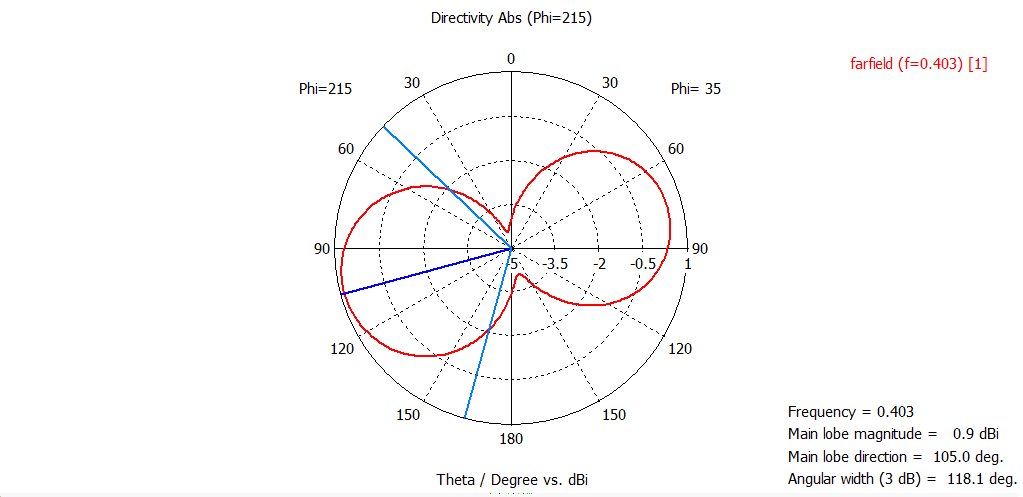
\includegraphics[scale=0.6]{./Simulaciones/tunned_antenna/tunned_serpentine_antenna_radiation_pattern}}
    \subfigure[]{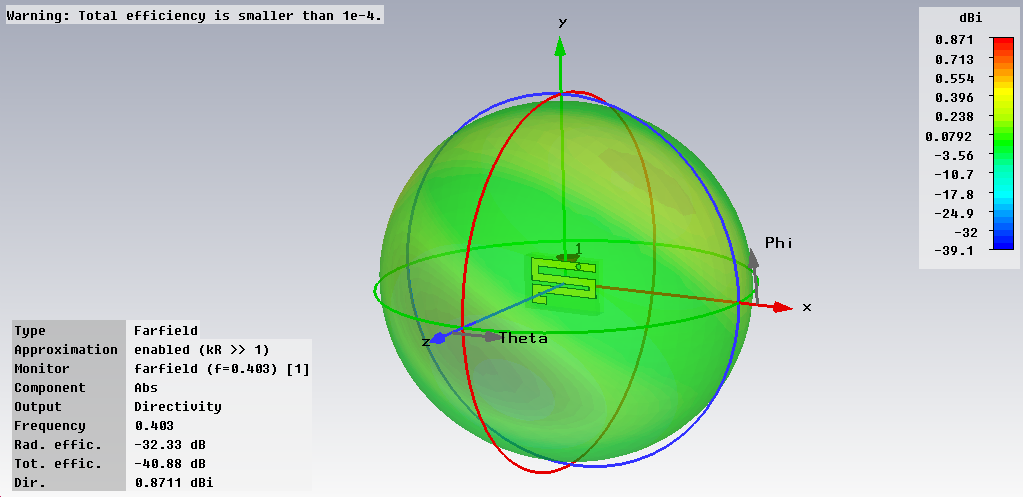
\includegraphics[scale=0.6]{./Simulaciones/tunned_antenna/tunned_serpentine_antenna_radiation_pattern_3D}}
    \caption{Representación del diagrama de radiación de la antena modificada en espacio libre. En (a) coordenadas polares en 2D manteniendo $\phi$ = 215º y en (b) en 3D, donde podemos ver la advertencia del programa en cuanto a la radiación efectiva.}
    \label{fig:fig5.21}
\end{figure}

\clearpage

\subsection{Antena modificada rodeada de músculo}\label{subsec:antena-modificada-rodeada-de-musculo}

Esta sección es importante ya que veremos si nuestro diseño modificado a partir del propuesto en el artículo ofrece mejores resultados con las condiciones de simulación que tenemos. La única novedad respecto a la sección anterior es que rodeamos nuestra antena de un bloque de músculo.

% ANTENA MODIFICADA MUSCULO
\begin{figure}[!htb]
    \centering
    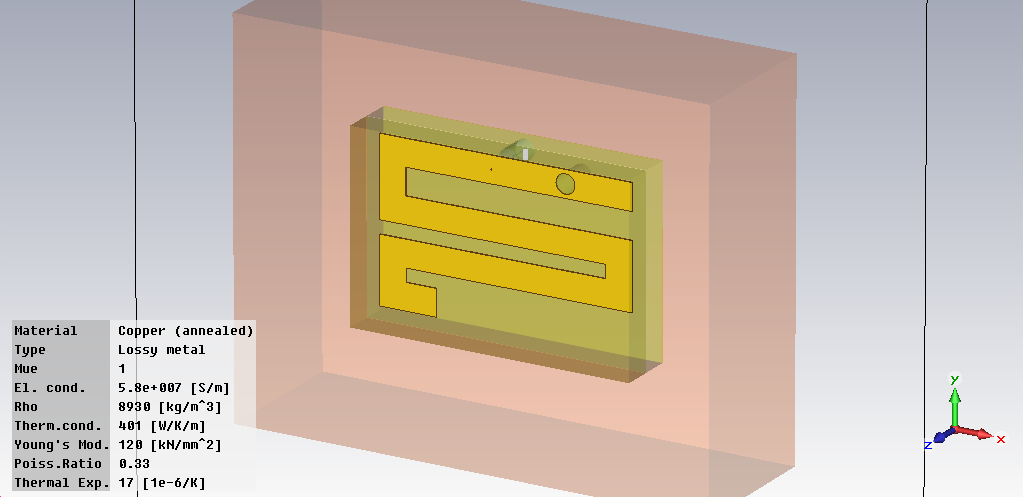
\includegraphics[scale=0.45]{./Simulaciones/tunned_antenna_muscle/tunned_serpentine_muscle}
    \caption{Diseño de la antena modificada rodeada de un bloque de músculo.}
    \label{fig:fig5.22}
\end{figure}

Los resultados del parámetro $S_{11}$ mejoran a los simulados anteriormente en la misma condición con bloque de músculo. Se obtiene un valor de -41.7 dB en la banda MICS tal y como se aprecia en la \textit{fig. \ref{fig:fig5.23}}. El dato es muy positivo para nuestro proyecto y para nuestro conjunto de simulaciones.

% S11 ANTENA MODIFICADA MUSCULO
\begin{figure}[!htb]
    \centering
    \subfigure[]{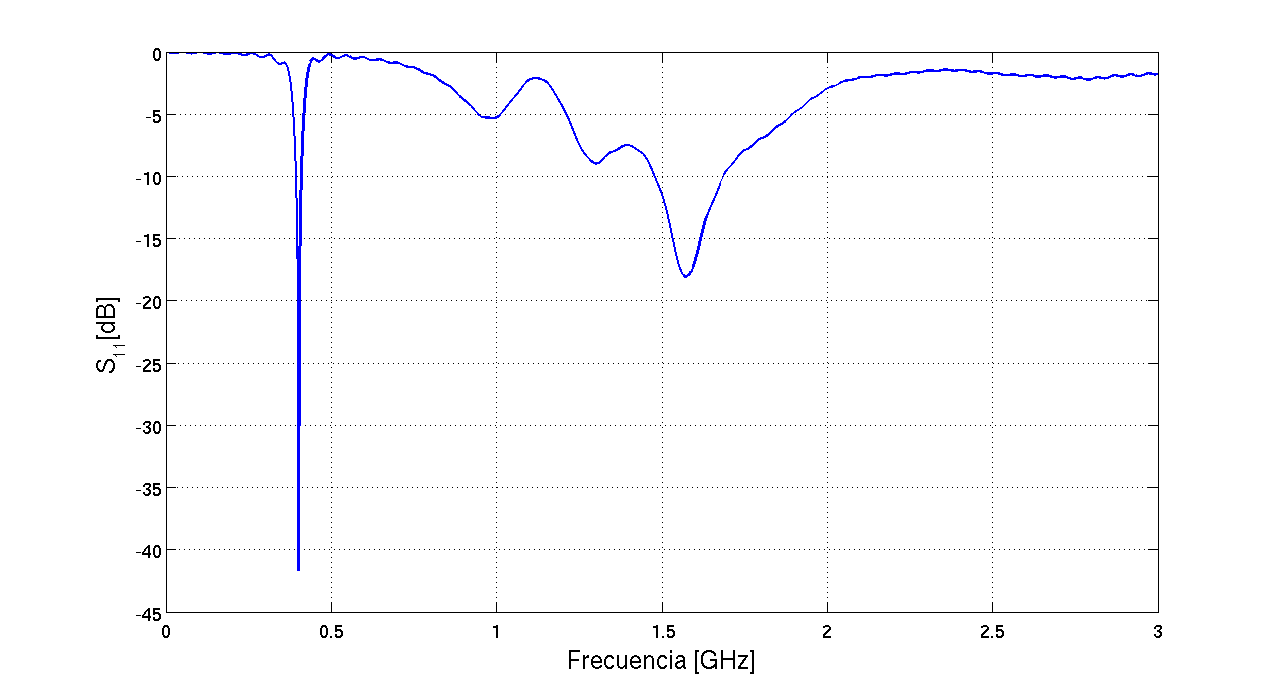
\includegraphics[scale=0.45]{./Simulaciones/matlab2/S11_tunned_muscle}}
    \subfigure[]{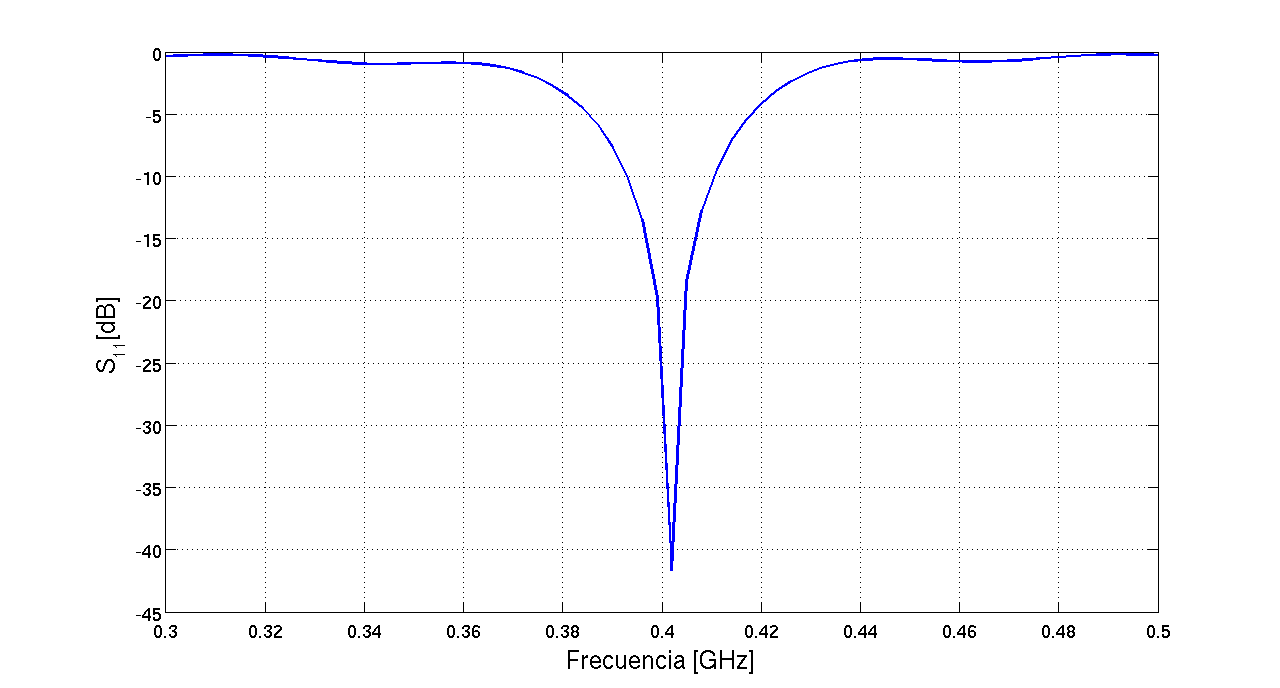
\includegraphics[scale=0.45]{./Simulaciones/matlab2/S11_tunned_muscle_zoom}}
    \caption{Gráficas que recogen el parámetro $S_{11}$ de la antena de serpentina modificada en tejido muscular. En (a) medidas simuladas de 0 a 3 GHz y en (b) se ha aplicado un zoom en la banda MICS.}
    \label{fig:fig5.23}
\end{figure}

El valor de -41.7 dB es mejor que el anterior dato obtenido en el mismo entorno de simulación (-3.02 dB en la banda MICS). Nos indica que nuestra antena modificada supera en el parámetro $S_{11}$ a la antena que hemos simulado a partir del artículo. Uno de los inconvenientes encontrados es el reducido ancho de banda, debido al grosor del substrato, pero tampoco podemos aumentarlo más, porque perderíamos eficiencia en radiación. Otra desventaja importante es en el caso de construir la antena de manera fisica: será muy difícil conseguir estos valores, seguramente nos lo impidan el uso de la conexión directa por cable coaxial o por algún fallo o error en la construcción de la antena, es decir, impurezas al cortar los materiales o imperfecciones de los mismos.

\clearpage

En comparación con la simulación obtenida con la antena original en músculo, tenemos mejor valor de $S_{11}$ y una frecuencia centrada en la banda MICS.

\begin{figure}[!htb]
    \centering
    \subfigure[]{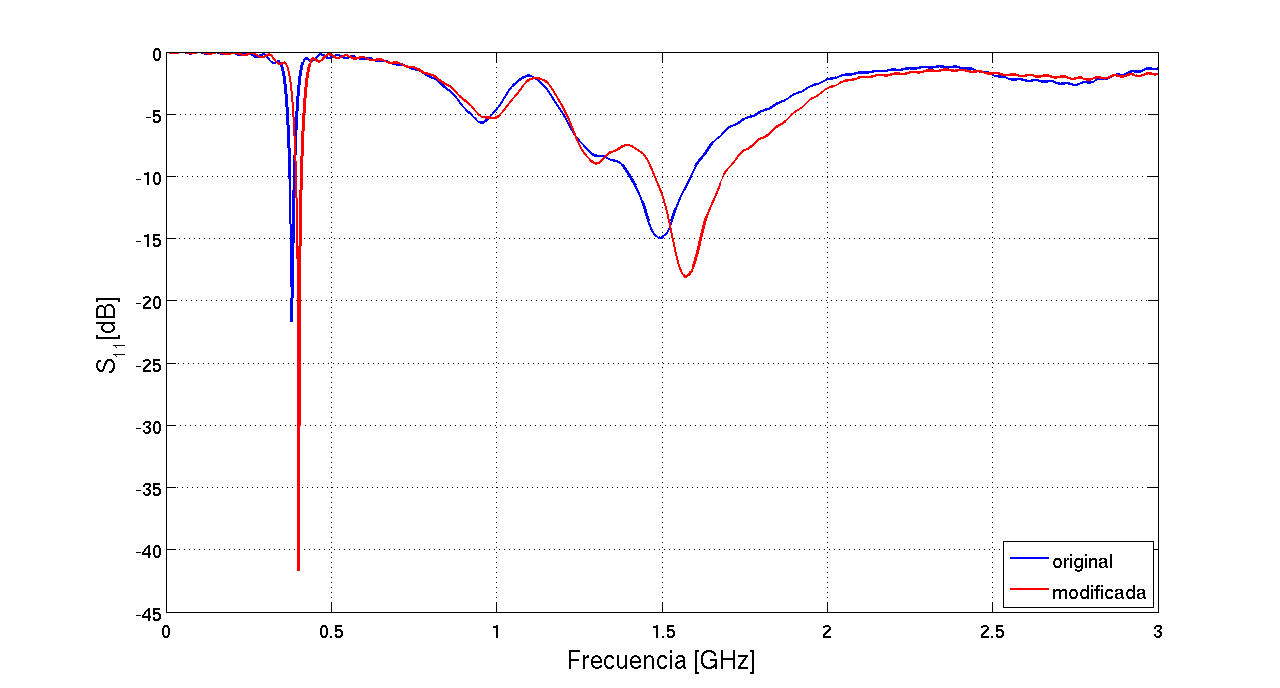
\includegraphics[scale=0.4]{./Simulaciones/matlab2/S11_vs_original_tunned_muscle}}
    \subfigure[]{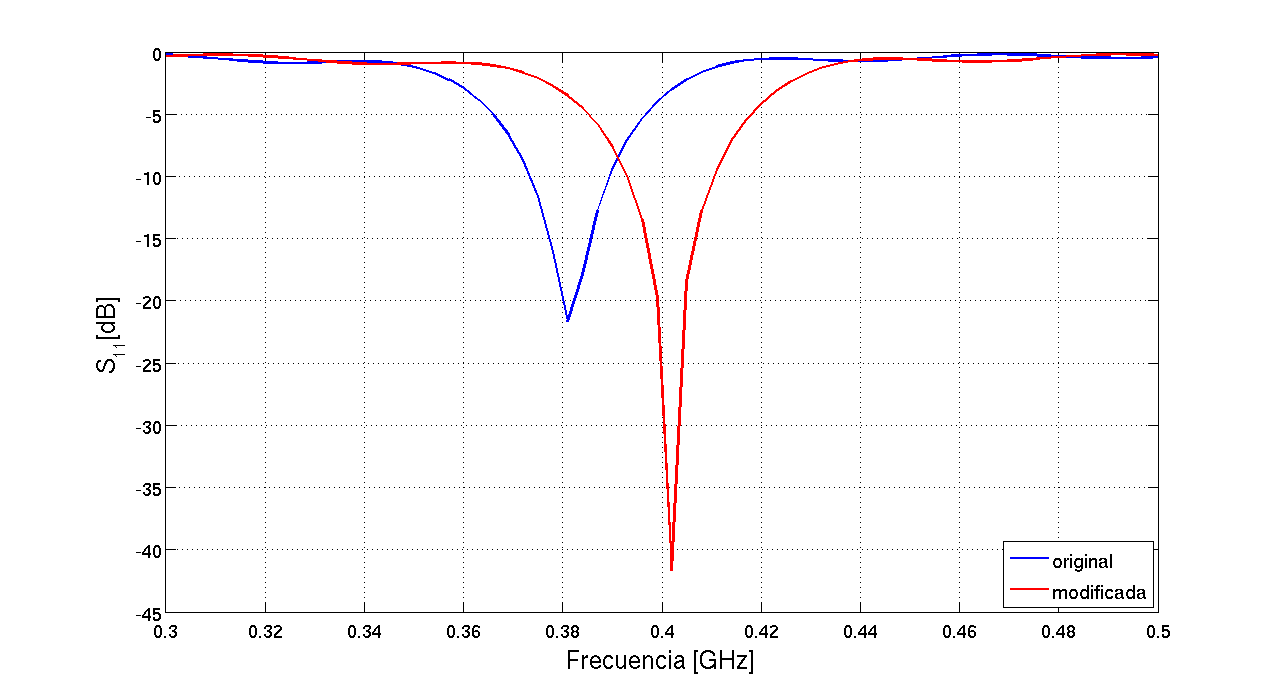
\includegraphics[scale=0.4]{./Simulaciones/matlab2/S11_vs_original_tunned_muscle_zoom}}
    \caption{Comparación parámetro $S_{11}$ de la antena original y la modificada en músculo. En (a) barrido de frecuencias de 0 a 3 GHz y en (b) zoom en la banda MICS.}
    \label{fig:fig5.24}
\end{figure}

\clearpage

A continuación, mostraremos el campo eléctrico de nuestra antena modificada en las \textit{figs. \ref{fig:fig5.25}},~\textit{\ref{fig:fig5.26}},~\textit{\ref{fig:fig5.27}} y~\textit{\ref{fig:fig5.28}}.

% E FIELD ANTENA MODIFICADA MUSCULO
\begin{figure}[!htb]
    \centering
    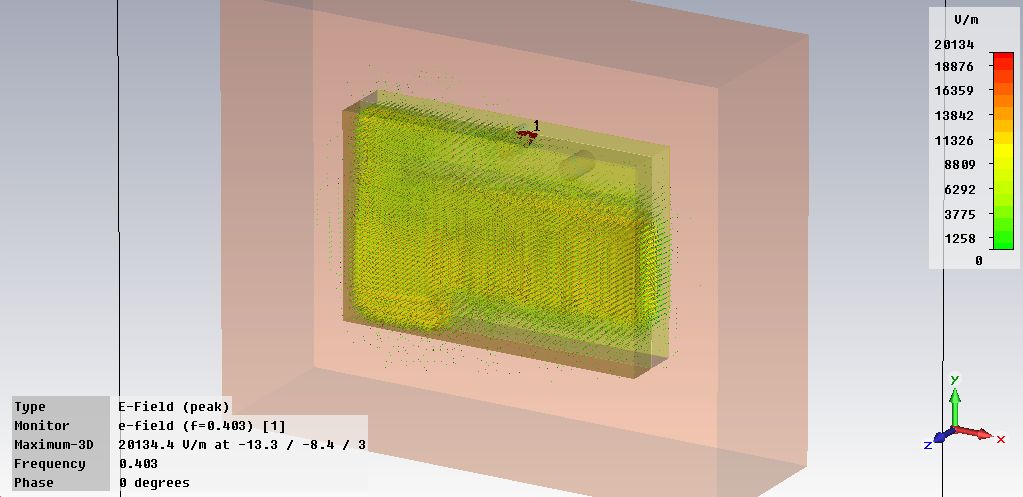
\includegraphics[scale=0.4]{./Simulaciones/tunned_antenna_muscle/tunned_serpentine_muscle_E-Field}
    \caption{Representación campo eléctrico en prespectiva.}
    \label{fig:fig5.25}
\end{figure}

\begin{figure}[!htb]
    \centering
    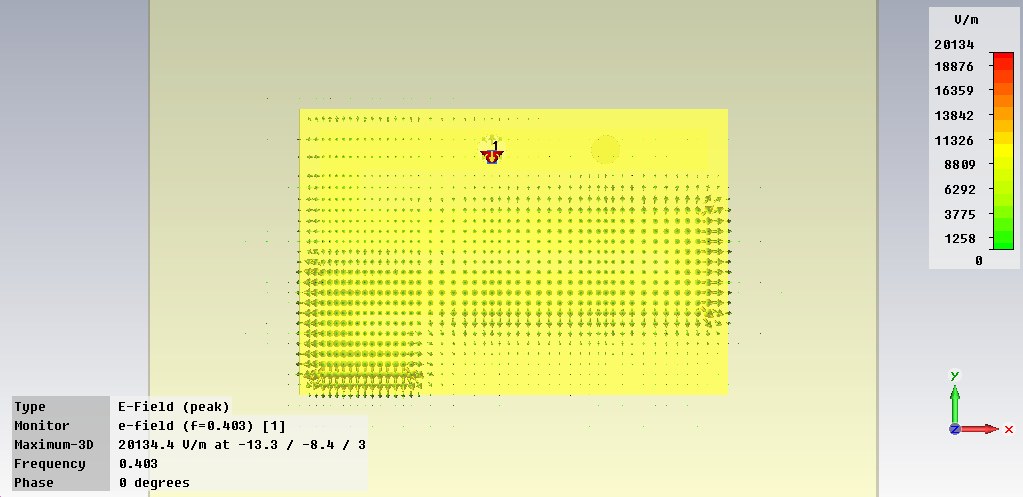
\includegraphics[scale=0.4]{./Simulaciones/tunned_antenna_muscle/tunned_serpentine_muscle_E-Field_2}
    \caption{Representación campo eléctrico desde el frente.}
    \label{fig:fig5.26}
\end{figure}

\begin{figure}[!htb]
    \centering
    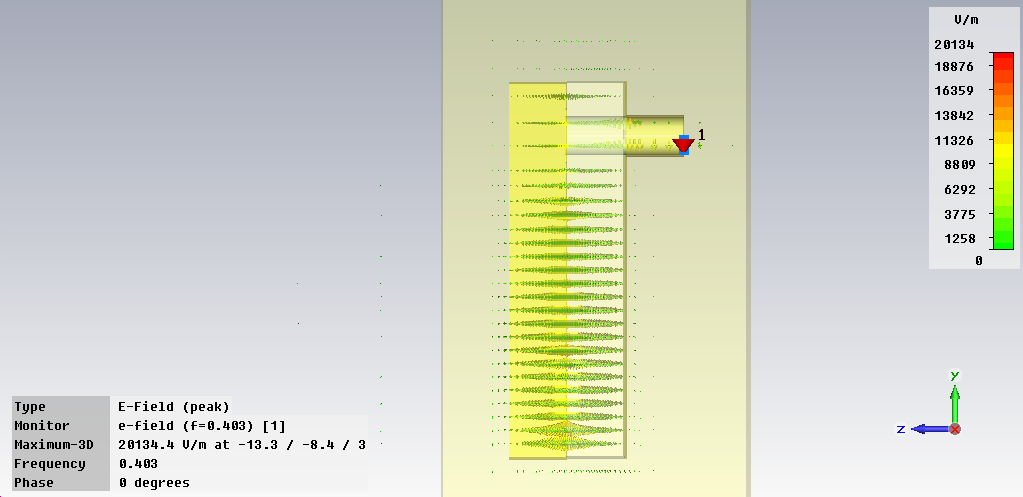
\includegraphics[scale=0.4]{./Simulaciones/tunned_antenna_muscle/tunned_serpentine_muscle_E-Field_3}
    \caption{Representación campo eléctrico desde el lado derecho.}
    \label{fig:fig5.27}
\end{figure}

\begin{figure}[!htb]
    \centering
    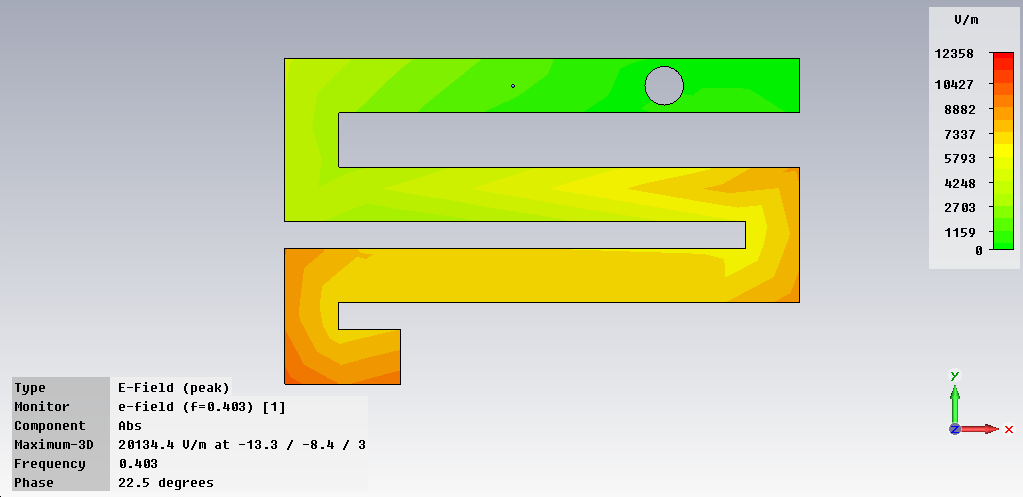
\includegraphics[scale=0.4]{./Simulaciones/tunned_antenna_muscle/tunned_serpentine_muscle_E-Field_4}
    \caption{Representación campo eléctrico en el parche radiante.}
    \label{fig:fig5.28}
\end{figure}

En las \textit{figs. \ref{fig:fig5.25}},~\textit{\ref{fig:fig5.26}},~\textit{\ref{fig:fig5.27}} y~\textit{\ref{fig:fig5.28}} anteriores hemos podido comprobar cómo se distribuye el campo en la antena. Sucede al igual que antes, la mayoría del campo eléctrico se dispone en la parte baja del parche y sale al exterior así, generando los \textit{fringing fields} u ondas viajeras, que son las que hacen que una antena funcione y radie. La posición del pin de tierra junto al de alimentación son clave para conseguir la frecuencia de resonancia a la que trabajamos y conseguir estos campos.

La distribución de pérdida de potencia se muestra en la \textit{fig. \ref{fig:fig5.29}}.

% PÉRDIDA DE POTENCIA ANTENA MODIFICADA MÚSCULO
\begin{figure}[!htb]
    \centering
    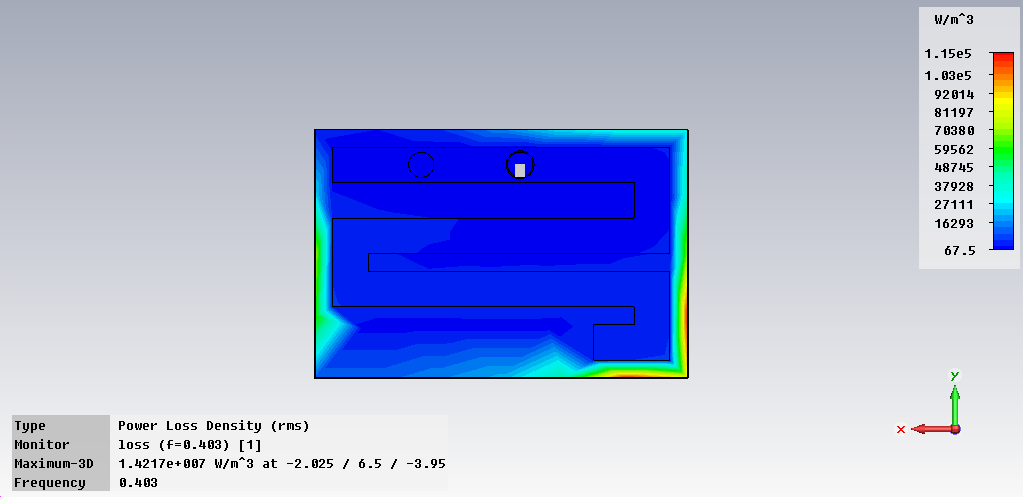
\includegraphics[scale=0.5]{./Simulaciones/tunned_antenna_muscle/tunned_serpentine_muscle_power_loss}
    \caption{Representación de la pérdida de potencia en el dieléctrico.}
    \label{fig:fig5.29}
\end{figure}

Al igual que sucedía con la antena original, la potencia se pierde por los lados más bajos del dieléctrico. Quizá esto pueda ser también un punto de estudio para conseguir una antena que consiga una eficiencia energética mayor, sin tener muchas pérdidas por ondas reflejadas u ondas superficiales.

El diagrama de radiación de nuestra antena modificada resulta muy parecido al de la antena original. Sin embargo, hemos perdido ganancia en la antena, seguramente debido a la disminución del parámetro $S_{11}$. Otro punto de estudio interesante sería conseguir un compromiso entre la ganancia de la antena y el parámetro $S_{11}$.

% DIAGRAMA DE RADIACIÓN ANTENA MODIFICADA MÚSCULO
\begin{figure}[!htb]
    \centering
    \subfigure[]{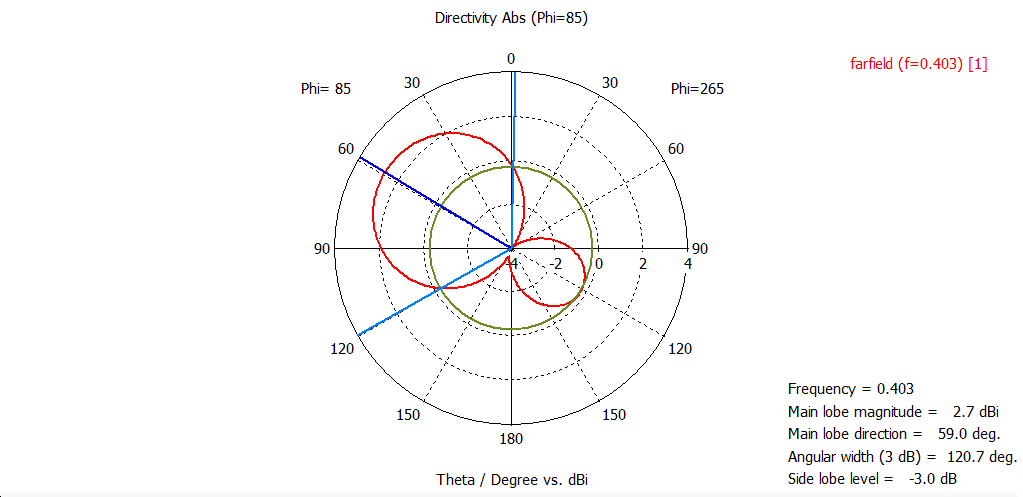
\includegraphics[scale=0.5]{./Simulaciones/tunned_antenna_muscle/tunned_serpentine_muscle_radiation_pattern}}
    \subfigure[]{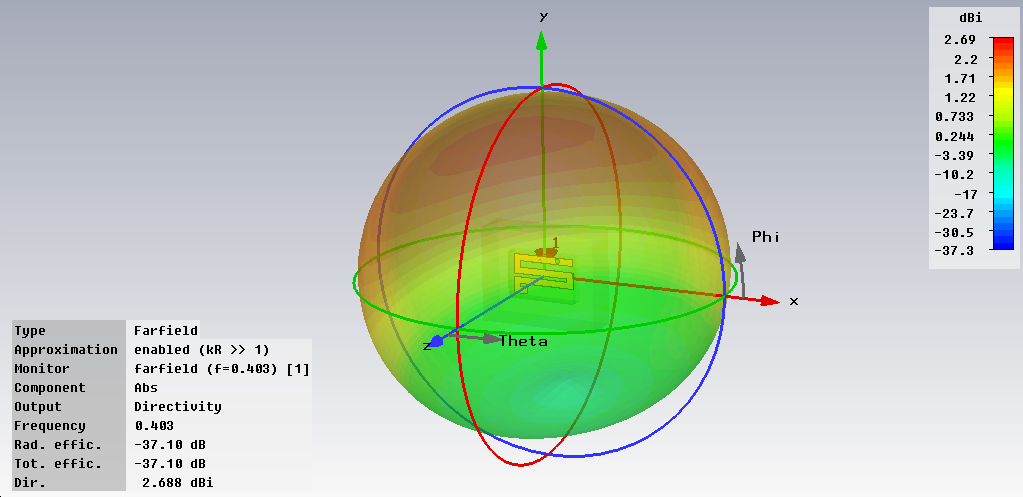
\includegraphics[scale=0.5]{./Simulaciones/tunned_antenna_muscle/tunned_serpentine_muscle_radiation_pattern_3D}}
    \caption{Representación del diagrama de radiación de la antena modificada en tejido muscular. En (a) coordenadas polares en 2D manteniendo $\phi$ = 85º y en (b) en 3D.}
    \label{fig:fig5.30}
\end{figure}

El lóbulo principal se establece a unos 60º $\theta$, recayendo toda la radiación hacia la parte superior de la antena, como podemos apreciar en la imagen en 3D \textit{fig. \ref{fig:fig5.30} (b)}: la zona roja. En definitiva, se ha conseguido un ancho de haz de 120º. Una simulación posterior a esta podría ser comprobar la corriente superficial en el parche en dos antenas iguales a nuestra antena modificada: una haciendo de transmisor y otra de receptor, para comprobar el \textit{teorema de reciprocidad} con esta antena, el cual establece que cualquier dispositivo que radie potencia en forma de ondas electromagnéticas, una antena en términos coloquiales, funciona igualmente como transmisor y como receptor.

\subsection{Antena modificada rodeada de tres capas de tejido: piel, grasa y músculo}\label{subsec:3capas}

Nuestra antena modificada parece eficiente según estas simulaciones mostradas anteriormente. Ahora bien, ¿y si simulamos nuestra antena en un entorno más real?, es decir, ¿con más tejidos corporales? El artículo de referencia hace experimentos además de con músculo, con otros tipos de tejidos. En nuestro caso, con la antena modificada, vamos a simular en un entorno más realista: colocaremos la antena en un entorno electromagnético consistente en tres capas, piel, grasa y músculo. Podemos ver este diseño en la \textit{fig. \ref{fig:fig5.31}}.

% ANTENA MODIFICADA 3 CAPAS
\begin{figure}[!htb]
    \centering
    \subfigure[]{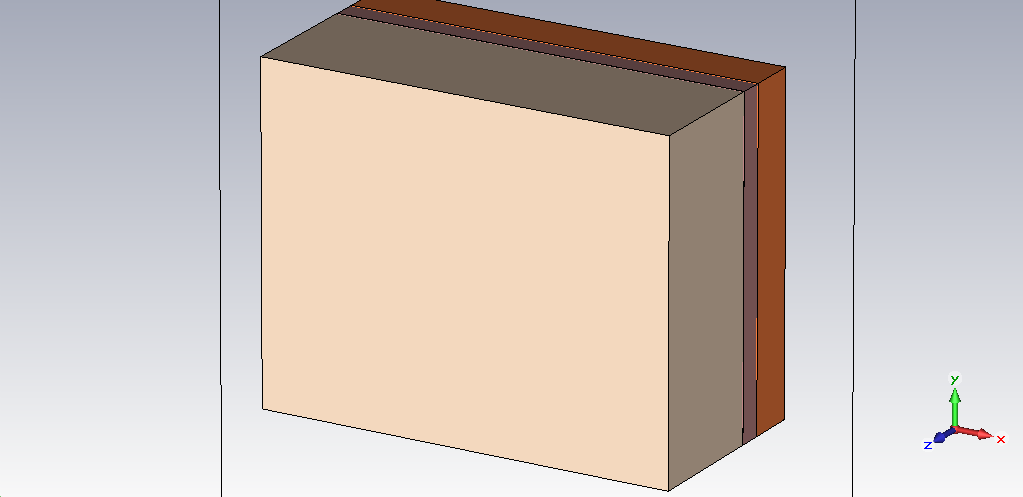
\includegraphics[scale=0.5]{./Simulaciones/tunned_antenna_3layers/tunned_serpentine_3layers}}
    \subfigure[]{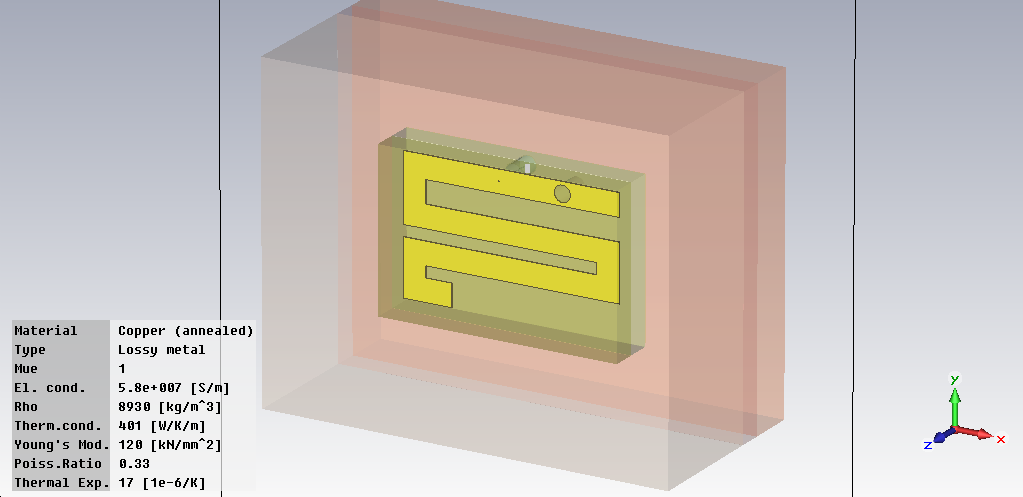
\includegraphics[scale=0.5]{./Simulaciones/tunned_antenna_3layers/tunned_serpentine_3layers_2}}
    \caption{Representación de la antena modificada en el entorno dieléctrico de tres capas: piel, grasa y músculo. En (a) vista general con orden de capas desde el frente hacia atrás: piel, grasa y músculo. En (b) vista de la antena introducida entre las tres capas.}
    \label{fig:fig5.31}
\end{figure}

% TABLA CONB MEDIDAS BLOQUE DE TRES CAPAS

Las medidas y carcaterísticas de los materiales del bloque diseñado de tres capas se recogen en la tabla siguiente:

% Tabla medidas bloque 3 capas
% Piel. Largo = 50 mm,alto = 40 mm,ancho = 14 mm, E_r = 31.29, Conductividad = 8.0138 S/m
% Grasa. Largo = 50 mm,alto = 40 mm,ancho = 3 mm, E_r = 4.6023, Conductividad = 0.58521 S/m
% Músculo. Largo 50 mm= ,alto = 40 mm,ancho = 6 mm, E_r = 42.807, Conductividad = 0.6463 S/m

\begin{table}[h]
    \centering\scalebox{0.99}{
        \begin{tabular}{| c | c | c | c | c | c |}
            \hline
            \textbf{Material} & \textbf{Dimensiones} & \textbf{Permitividad} & \textbf{Conductividad}   \\
            & \textbf{[mm]}        & \textbf{relativa}     & \textbf{eléctrica [S/m]} \\
            \hline
            \hline
            \textbf{Piel}     & 50 x 40 x 14         & 31.29                 & 8.0138                   \\
            \hline
            \hline
            \textbf{Grasa}    & 50 x 40 x 3          & 4.6023                & 0.58521                  \\
            \hline
            \hline
            \textbf{Músculo}  & 50 x 40 x 6          & 42.807                & 0.6463                   \\
            \hline
            \hline
        \end{tabular}}
    \caption{Propiedades del bloque de tres capas (piel, grasa y músculo) diseñado para la simulación.}
    \label{tab:tabla5.5}
\end{table}

En cuanto al parámetro $S_{11}$, de nuevo ha sido modificado y no está centrado en la banda MICS, aunque tiene buenas propiedades para ella. Por supuesto, ha influido el nuevo entorno dieléctrico en el que nos encontramos, ya no es una única permitividad relativa $\epsilon_{r}$: ahora hay tres y muy distintas todas ellas. Dicho desplazamiento podemos verlo en las \textit{figs. \ref{fig:fig5.32} (a)} y \textit{(b)}.

% S11 ANTENA MODIFICADA 3 CAPAS
\begin{figure}[!htb]
    \centering
    \subfigure[]{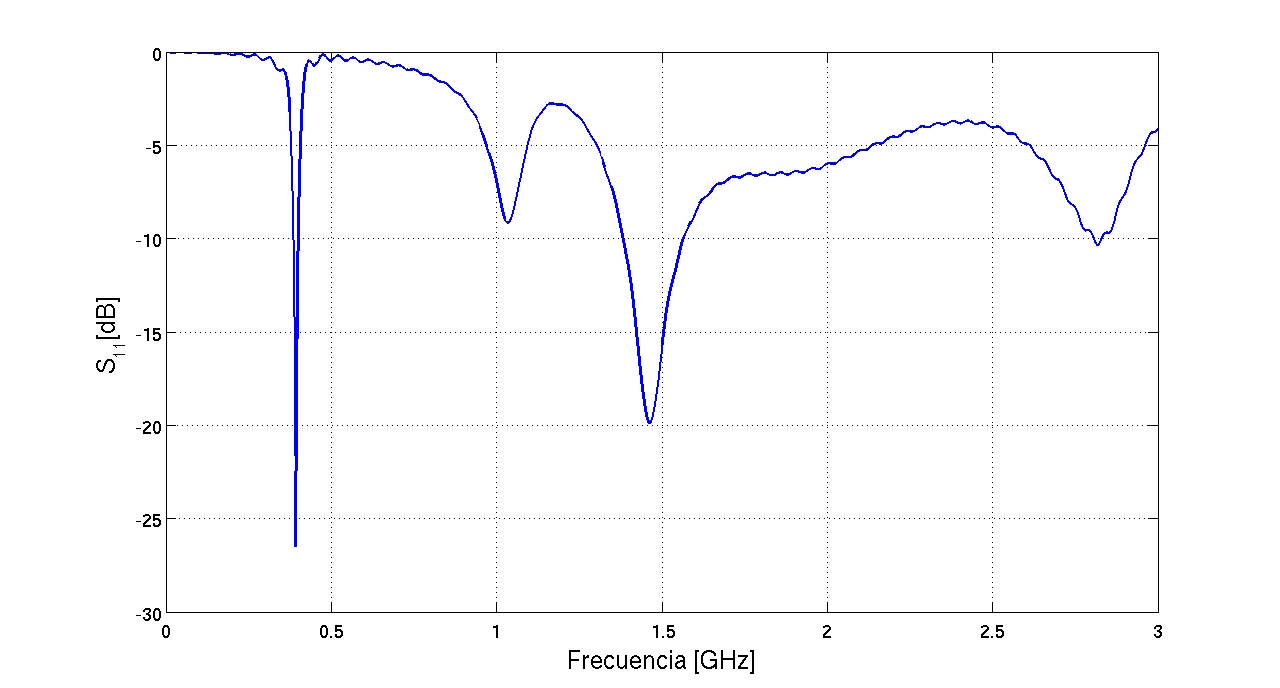
\includegraphics[scale=0.45]{./Simulaciones/matlab2/S11_tunned_3layers}}
    \subfigure[]{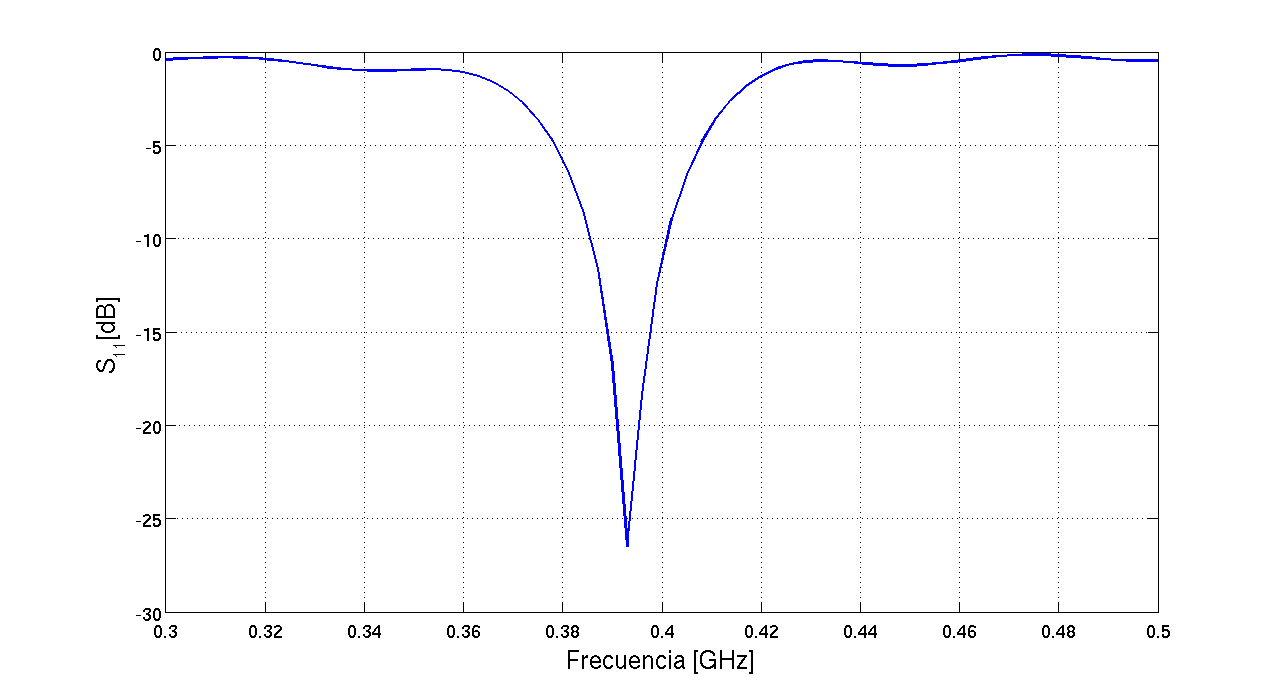
\includegraphics[scale=0.45]{./Simulaciones/matlab2/S11_tunned_3layers_zoom}}
    \caption{Gráficas que recogen el parámetro $S_{11}$ de la antena modificada en de tres capas. En (a) medidas simuladas de 0 a 3 GHz y en (b) se ha aplicado un zoom en la banda MICS.}
    \label{fig:fig5.32}
\end{figure}

Para la banda MICS, tenemos -7.74 dB $\simeq$ -8 dB, lo cual está razonablemente bien para un simulación que asemeja un entorno real. Un punto de estudio también interesante sería modificar esta antena, a partir de la que tenemos, para que trabaje perfectamente en la banda MICS.

\clearpage

En comparación con la simulación en músculo, nuestro mínimo $S_{11}$ se desplaza a una frecuencia menor, 393 MHz: representado en \textit{figs. \ref{fig:fig5.32} (b)} y~\textit{\ref{fig:fig5.33}}.

\begin{figure}[!htb]
    \centering
    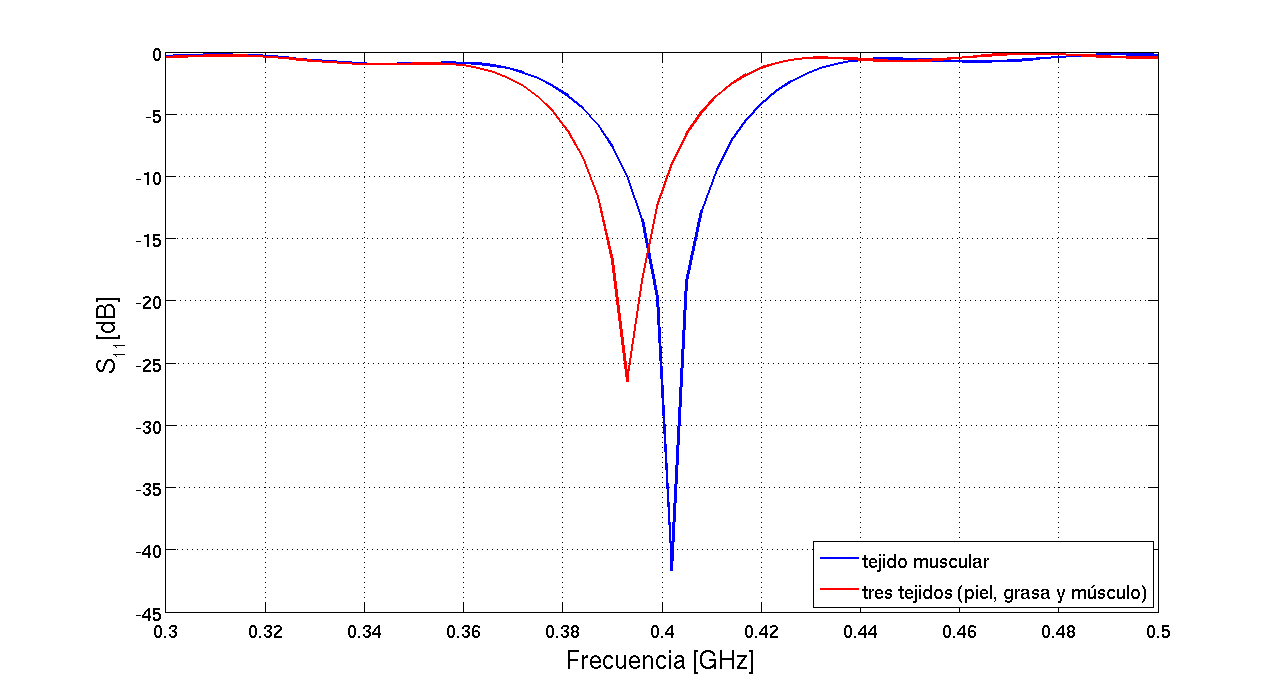
\includegraphics[scale=0.45]{./Simulaciones/matlab2/S11_vs_tunned_3layers_muscle_zoom}
    \caption{Gráfica comparativa del parámetro $S_{11}$ entre la antena modificada simulada en músculo y con tres capas de tejido.}
    \label{fig:fig5.33}
\end{figure}

La posible razón del desplazamiento sufrido es debido al cambio de entorno dieléctrico. En la anterior simulación, la antena está rodeada completamente de tejido muscular y en esta ocasión, la antena está rodeada en su mayoría por el tejido de piel. Aún así, es razonable pensar que la antena funcionaría mejor en la banda MICS si se corrigieran estos defectos, modificando el parche radiante o los materiales.\\

El campo eléctrico radiado en esta situación nos lo muestra la \textit{fig. \ref{fig:fig5.34}}. No ha habido grandes cambios con respecto a las simulaciones anteriores, pero se asemejan mucho más a las simulaciones en tejido muscular que en espacio libre.

% E FIELD ANTENA MODIFICADA 3 CAPAS
\begin{figure}[!htb]
    \centering
    \subfigure[]{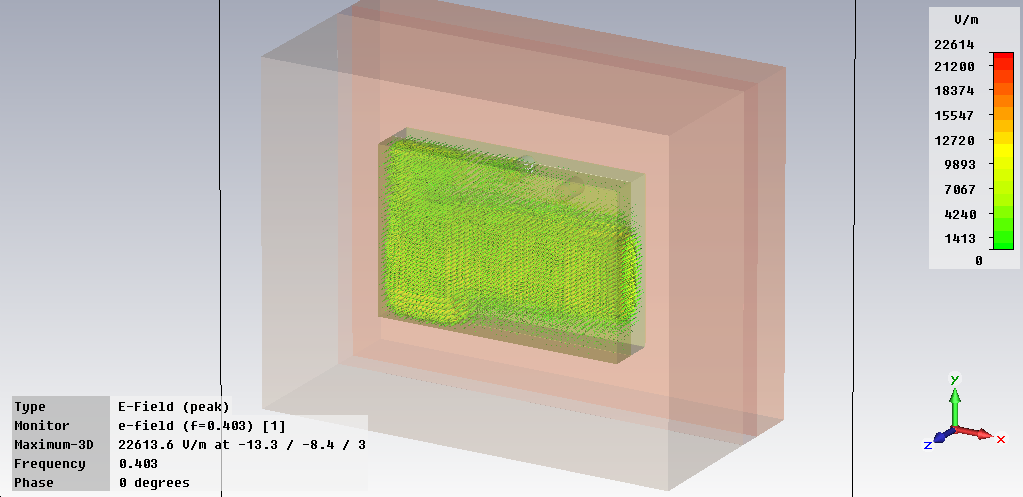
\includegraphics[scale=0.32]{./Simulaciones/tunned_antenna_3layers/tunned_serpentine_3layers_E-Field}}
    \subfigure[]{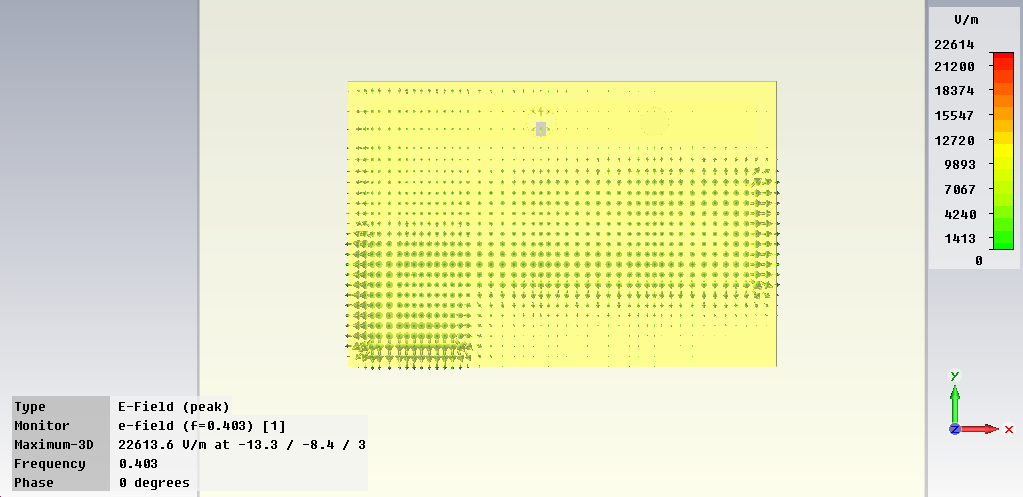
\includegraphics[scale=0.32]{./Simulaciones/tunned_antenna_3layers/tunned_serpentine_3layers_E-Field_2}}
    \subfigure[]{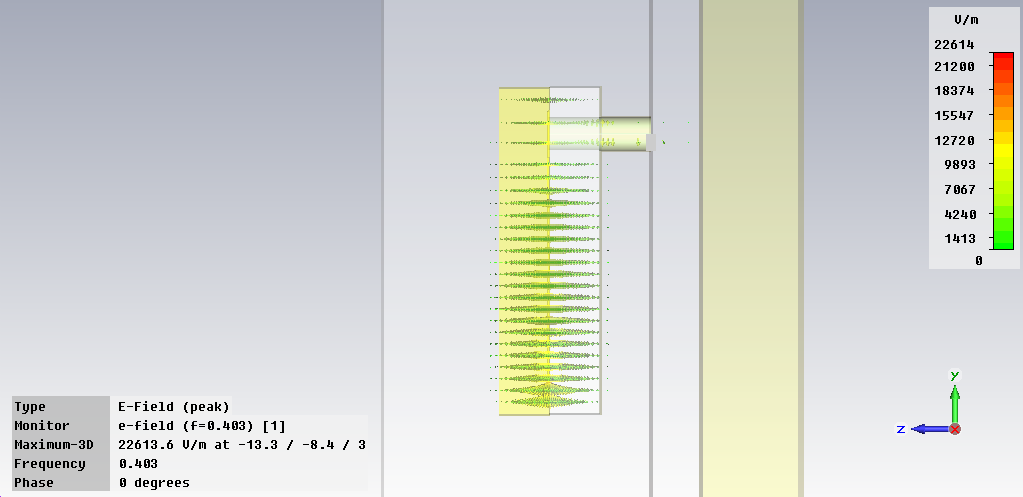
\includegraphics[scale=0.32]{./Simulaciones/tunned_antenna_3layers/tunned_serpentine_3layers_E-Field_3}}
    \subfigure[]{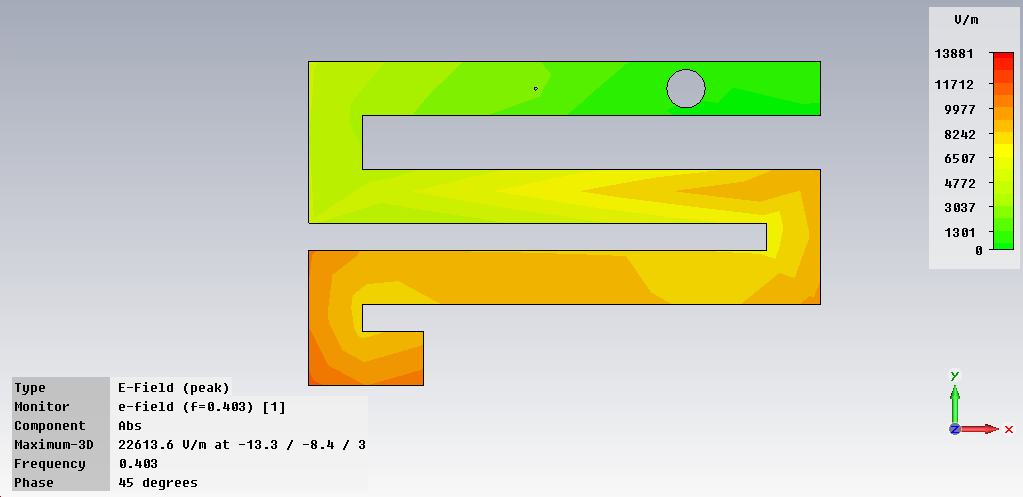
\includegraphics[scale=0.32]{./Simulaciones/tunned_antenna_3layers/tunned_serpentine_3layers_E-Field_4}}
    \caption{Representación del campo eléctrico en distintas vistas para la antena modificada en el entorno de tres capas. En (a) vista en prespectiva; en (b) vista frontal; en (c) vista desde el lado derecho y en (d) vista del parche radiante.}
    \label{fig:fig5.34}
\end{figure}

\clearpage

El diagrama de radiación de este modelo se ve en la \textit{fig. \ref{fig:fig5.35}}:

% DIAGRAMA DE RADIACIÓN ANTENA MODIFICADA 3 CAPAS
\begin{figure}[!htb]
    \centering
    \subfigure[]{\includegraphics[scale=0.4]{./Simulaciones/tunned_antenna_3layers/tunned_serpentine_3layers_radiation_pattern}}
    \subfigure[]{\includegraphics[scale=0.4]{./Simulaciones/tunned_antenna_3layers/tunned_serpentine_3layers_radiation_pattern_3D}}
    \caption{Representación del diagrama de radiación de la antena modificada en tejido muscular. En (a) coordenadas polares en 2D manteniendo $\phi$ = 90º y en (b) en 3D, donde podemos ver la advertencia del programa en cuanto a la radiación efectiva.}
    \label{fig:fig5.35}
\end{figure}

Las imágenes nos muestran dos lóbulos, el principal y el posterior muy similares a los vistos en tejido muscular. El ancho de haz a 3 dB en este caso es un poco mayor, pero lo encontramos a los mismos 60º $\theta$.

Como podemos comprobar, la radiación efectiva es muy pobre, está por debajo de los -40 dB, por lo que el diseño de la antena ha de ser modificado bastante más si queremos que funcione a la perfección dentro de un entorno de piel, grasa y músculo. Únicamente se ha modificado como se vió en la sección anterior los parámetros del parche, las medidas \textit{B, C} y \textit{D}; por consiguiente, ha de modificarse y estudiarse otros parámetros como las propias medidas de la antena o el grosor de los capas dieléctricas o los materiales, etc. Para simplificar nuestro proyecto y por diversas limitaciones que mencionaremos más adelante, se ha buscado eficiencia exclusivamente en entornos con tejido muscular.

Al igual que venimos diciendo a lo largo de este capítulo, hay diversos puntos de estudio que se pueden engrosar dentro de una serie de líneas futuras de trabajo a partir del estudio plasmado en estas hojas. Basándonos en nuestro diseño modificado se puede por ejemplo, mejorar la eficiencia de la antena, otros tipos de conectores, mejorar las prestaciones para entornos multicapa, etc.


\section{Diseño optimizado de la antena de serpentina propuesta con nuevos materiales}\label{sec:optimizado}

En este apartado vamos a buscar la eficiencia de nuestra antena con nuevos materiales. El motivo de los nuevos materiales tiene su razón en que son materiales muy utilizados y muy habituales en laboratorios que fabrican dispositivos eléctricos. Son además materiales que poseen características parecidas a los materiales propuestos en el artículo. Los materiales originales dieléctricos, \textit{Macor} y \textit{Alumina}, han sido sustituidos por los recogidos en la \textit{tabla \ref{tab:tabla5.6}}:

% Tabla con materiales nuevos

\begin{table}[h]
    \centering\scalebox{0.99}{
        \begin{tabular}{| c | c | c | c | c | c |}
            \hline
            \textbf{Materiales dieléctricos}           & \textbf{$\epsilon_{r}$} & Grosor [mm] \\
            \hline
            \hline
            Arlon 1000 (substrato)                     & 10                      & 2.54        \\
            \hline
            Policloruro de vinilo (PVC) (superestrato) & 3.19                    & 3           \\
            \hline
            \hline
            \textbf{Parche, masa y conectores}         & \textbf{$\sigma$ [S/m]} & Grosor [mm] \\
            \hline
            \hline
            Cobre                                      & 5.8 · $10^7$            & 0.1         \\
            \hline
            \hline
        \end{tabular}}
    \caption{Materiales nuevos para la antena de serpentina adaptada del artículo de Soontornpipit.}
    \label{tab:tabla5.6}
\end{table}

Como podemos observar en la \textit{tabla \ref{tab:tabla5.6}}, se ha modificado el grosor de la capa del substrato, que pasa de 3 mm a 2.54 mm. Este cambio sucede porque los materiales disponibles en laboratorios vienen de fábrica con unos espesores fijos y en el caso de \textit{Arlon 1000}, este espesor es de 1.27 mm. Al poner dos capas de este material, hemos obtenido un grosor de 2.54 mm, un valor cercano a los 3 mm originales.

Al igual que sucede en la anterior sección con el diseño modificado, aquí también debemos rediseñar las dimensiones del parche radiante. Cabe indicar que las dimensiones de la antena son idénticas de nuevo, por lo que lo único que se va a modificar son las dimensiones del parche y el grosor de la capa del substrato. La \textit{tabla \ref{tab:tabla5.7}} recoge los parámetros que han sido cambiados y la evolución hasta conseguir un parámetro $S_{11}$ eficiente.

\begin{table}[h]
    \centering\scalebox{0.85}{
        \begin{tabular}{| c | c | c | c | c | c |}
            \hline
            %\fcolorbox{orange}{orange}{ \color{white} LaTeX}
            \textbf{Parámetro modificado} & \textbf{Frecuencia de resonancia} & \textbf{Parámetro $S_{11}$} & \textbf{Ganancia} \\
            \hline
            \hline
            B = 6 mm                      &                                   &                             &                                     \\
            C = 7.8 mm                    & 384 MHz                           & -30.69 dB                   & 2.7 dBi                             \\
            D = 7 mm                      &                                   &                             &                                     \\
            \hline
            B = 6 mm                      &                                   &                             &                                     \\
            C = 7.8 mm                    & 396 MHz                           & -27.62 dB                   & 2.71 dBi                            \\
            D = 9 mm                      &                                   &                             &                                     \\
            \hline
            B = 6 mm                      &                                   &                             &                                     \\
            C = 7.8 mm                    & 399 MHz                           & -30.7 dB                    & 2.73 dBi                            \\
            D = 9.5 mm                    &                                   &                             &                                     \\
            \hline
            B = 5.5 mm                    &                                   &                             &                                     \\
            C = 7.8 mm                    & 402 MHz                           & -25.55 dB                   & 2.76 dBi                            \\
            D = 9.5 mm                    &                                   &                             &                                     \\
            \hline
            B = 5.5 mm                    &                                   &                             &                                     \\
            C = 7.45 mm                   & 402 MHz                           & -28.39 dB                   & 2.735 dBi                           \\
            D = 9.5 mm                    &                                   &                             &                                     \\
            \hline
            \textbf{B = 5.5 mm}           &                                   &                             &                                     \\
            \textbf{C = 7.5 mm}           & \textbf{402 MHz}                  & \textbf{-28.69 dB}          & \textbf{2.738 dBi ($\theta$ = 85º)} \\
            \textbf{D = 9.5 mm}           &                                   &                             &                                     \\
            \hline
            \hline
        \end{tabular}}
    \caption{Pruebas realizadas para conseguir una antena optimizada con nuevos materiales a partir del diseño modificado de la antena de serpentina.}
    \label{tab:tabla5.7}
\end{table}

Los parámetros que utilizaremos aparecen destacados en la última fila de la tabla. Es visible que las prestaciones, al menos en simulación, de esta antena respecto a la antena modificada (con casi -42 dB de parámetro $S_{11}$) han empeorado en más de 10 dB. Sin duda, los nuevos materiales utilizados, junto al nuevo grosor del substrato, son los causantes de este nuevo parámetro de la antena. Aun así, hemos de decir que las prestaciones son buenas e incluso mejores que las analizadas en el artículo base de nuestra investigación. Con estos nuevos datos, materiales y forma de la serpentina, vamos a analizar las características de la antena como en las secciones anteriores.

El objetivo de encontrar la eficiencia de nuestra antena se tiene que basar en un entorno parecido a la realidad, por eso las simulaciones expuestas en las siguientes páginas se desarrollan ya en un bloque de músculo, al igual que las pruebas que se han realizado para encontrar las medidas óptimas del parche. La nueva forma de este último se contemplan en la \textit{fig. \ref{fig:fig5.36}}. Se distingue de las anteriores en que los pines de alimentación y de masa están más a la izquierda, debido a que el parámetro \textit{D} ha aumentado más, y que el último brazo del parche es un poco más largo también.

\begin{figure}[!htb]
    \centering
    \includegraphics[scale=0.4]{./Simulaciones/optimized_antenna_muscle/optimized_muscle}
    \caption{Antena optimizada con los nuevos materiales dentro de un bloque de músculo.}
    \label{fig:fig5.36}
\end{figure}

La gráfica del parámetro $S_{11}$ en la \textit{fig. \ref{fig:fig5.37}} destaca que la antena cumple la función de radiar en la banda de trabajo MICS. Sin embargo, con respecto a las otras simulaciones realizadas, se puede observar un cambio de este parámetro en las demás bandas de frecuencias que resta eficiencia a la antena. Es un inconveniente a considerar tras cambiar los materiales originales del diseño del artículo. Aunque hayamos perdido eficiencia, la simulación demuestra que nuestra antena es capaz de trabajar a la frecuencia de la banda MICS rodeada de tejido muscular. El siguiente paso a partir de aquí, como futura línea de investigación sería encontrar con estos materiales un diseño aún más eficiente.

El dato de -28.69 dB como $S_{11}$ a 402 MHz para una antena microstrip es bastante aceptable. Nuestro objetivo de analizar e intentar mejorar el diseño se ha conseguido en este punto.

\begin{figure}[!htb]
    \centering
    \subfigure[]{\includegraphics[scale=0.4]{./Simulaciones/matlab2/S11_optimized_muscle}}
    \subfigure[]{\includegraphics[scale=0.4]{./Simulaciones/matlab2/S11_optimized_muscle_zoom}}
    \caption{Gráficas que recogen el parámetro $S_{11}$ de la antena optimizada con nuevos materiales en tejido muscular. En (a) medidas simuladas de 0 a 3 GHz y en (b) se ha aplicado un zoom en la banda MICS.}
    \label{fig:fig5.37}
\end{figure}

%\textbf{\textcolor{red}{rojo}}

Ahora vamos a realizar la comparación de dicho parámetro con las anteriores simulaciones. Esto nos servirá para analizar nuestro trabajo y ver cómo cambia la simulación con los parámetros modificados.

\begin{figure}[!htb]
    \centering
    \subfigure[]{\includegraphics[scale=0.4]{./Simulaciones/matlab2/S11_vs_original_tunned_optimized_muscle}}
    \subfigure[]{\includegraphics[scale=0.4]{./Simulaciones/matlab2/S11_vs_original_tunned_optimized_muscle_zoom}}
    \caption{Gráfica comparativa del parámetro $S_{11}$ entre la antenas original, modificada y optimizada simulada en músculo. En (a) medidas simuladas de 0 a 3 GHz y en (b) se ha aplicado un zoom en la banda MICS.}
    \label{fig:fig5.38}
\end{figure}

Se puede apreciar en la \textit{fig. \ref{fig:fig5.38}} como las tres simulaciones son casi idénticas a excepción de que están desplazadas a lo largo del ancho de frecuencias simulado. La antena modificada, en color rojo, es la que mejor prestaciones tiene, aunque muy seguida de nuestra antena optimizada con nuevos materiales, en color verde. Las posibles bandas resiudales conseguidas alrededor de 1.5 GHz no presentan mayor problema en las simulaciones. Para nuestro objetivo, las podemos ignorar.\\

La simulación del campo eléctrico es nuestro siguiente paso en la simulación como en anteriores secciones. Queda representado en la siguiente figura:

\begin{figure}[!htb]
    \centering
    \subfigure[]{\includegraphics[scale=0.25]{./Simulaciones/optimized_antenna_muscle/E_Field_optimized_muscle}}
    \subfigure[]{\includegraphics[scale=0.25]{./Simulaciones/optimized_antenna_muscle/E_Field_optimized_muscle_front}}
    \subfigure[]{\includegraphics[scale=0.25]{./Simulaciones/optimized_antenna_muscle/E_Field_optimized_muscle_right}}
    \subfigure[]{\includegraphics[scale=0.25]{./Simulaciones/optimized_antenna_muscle/E_Field_optimized_muscle_patch}}
    \caption{Representación del campo eléctrico en distintas vistas para la antena optimizada con nuevos materiales en tejido muscular. En (a) vista en prespectiva; en (b) vista frontal; en (c) vista desde el lado derecho y en (d) vista del parche radiante.}
    \label{fig:fig5.39}
\end{figure}

Como bien podemos observar en la \textit{fig. \ref{fig:fig5.39}} el campo eléctrico es muy parecido a las otras simulaciones. Los últimos brazos del parche radiante son los que más intensidad de campo eléctrico registran. Para nuestro interés, sabemos que esta antena radia perfectamente en un entorno de músculo.\\

Las últimas figuras que nos quedan por mostrar de nuestra simulación son los diagramas de radiación. Con respecto a la antena modificada, apenas ha cambiado el dibujo, únicamente lo destacable es el descenso en radiación eficiente al exterior, cerca de 2 dB por debajo.

\begin{figure}[!htb]
    \centering
    \subfigure[2D]{\includegraphics[scale=0.5]{./Simulaciones/optimized_antenna_muscle/radiation_pattern_2D}}
    \subfigure[3D]{\includegraphics[scale=0.5]{./Simulaciones/optimized_antenna_muscle/radiation_pattern_3D}}
    \caption{Diagramas de radiación de la antena optimizada con nuevos materiales en un bloque de músculo.}
    \label{fig:fig5.40}
\end{figure}

En definitiva, nuestra última simulación confirma que hemos obtenido una antena eficiente para la banda MICS, con unas características razonables y que sin duda, serían mejores si los materiales fueran los originales u otros más acordes para este diseño.
